\documentclass[12pt]{article}
\usepackage[]{color}
%% maxwidth is the original width if it is less than linewidth
%% otherwise use linewidth (to make sure the graphics do not exceed the margin)
\makeatletter
\def\maxwidth{ %
	\ifdim\Gin@nat@width>\linewidth
	\linewidth
	\else
	\Gin@nat@width
	\fi
}
\makeatother

\definecolor{fgcolor}{rgb}{0.345, 0.345, 0.345}
\newcommand{\hlnum}[1]{\textcolor[rgb]{0.686,0.059,0.569}{#1}}%
\newcommand{\hlstr}[1]{\textcolor[rgb]{0.192,0.494,0.8}{#1}}%
\newcommand{\hlcom}[1]{\textcolor[rgb]{0.678,0.584,0.686}{\textit{#1}}}%
\newcommand{\hlopt}[1]{\textcolor[rgb]{0,0,0}{#1}}%
\newcommand{\hlstd}[1]{\textcolor[rgb]{0.345,0.345,0.345}{#1}}%
\newcommand{\hlkwa}[1]{\textcolor[rgb]{0.161,0.373,0.58}{\textbf{#1}}}%
\newcommand{\hlkwb}[1]{\textcolor[rgb]{0.69,0.353,0.396}{#1}}%
\newcommand{\hlkwc}[1]{\textcolor[rgb]{0.333,0.667,0.333}{#1}}%
\newcommand{\hlkwd}[1]{\textcolor[rgb]{0.7te37,0.353,0.396}{\textbf{#1}}}%

%\usepackage{framed}
%\makeatletter
%\newenvironment{kframe}{%
%	\def\at@end@of@kframe{}%
%	\ifinner\ifhmode%
%	\def\at@end@of@kframe{\end{minipage}}%
%\begin{minipage}{\columnwidth}%
%	\fi\fi%
%	\def\FrameCommand##1{\hskip\@totalleftmargin \hskip-\fboxsep
%		\colorbox{shadecolor}{##1}\hskip-\fboxsep
%		% There is no \\@totalrightmargin, so:
%		\hskip-\linewidth \hskip-\@totalleftmargin \hskip\columnwidth}%
%	\MakeFramed {\advance\hsize-\width
%		\@totalleftmargin\z@ \linewidth\hsize
%		\@setminipage}}%
%{\par\unskip\endMakeFramed%
%	\at@end@of@kframe}
%\makeatother

\definecolor{shadecolor}{rgb}{.97, .97, .97}
\definecolor{messagecolor}{rgb}{0, 0, 0}
\definecolor{warningcolor}{rgb}{1, 0, 1}
\definecolor{errorcolor}{rgb}{1, 0, 0}
\newenvironment{knitrout}{}{} % an empty environment to be redefined in TeX

\usepackage{alltt} % use larger type; default would be 10pt

\usepackage[T5]{fontenc}
\usepackage[utf8]{inputenc} % set input encoding (not needed with XeLaTeX)

%%% Examples of Article customizations
% These packages are optional, depending whether you want the features they provide.
% See the LaTeX Companion or other references for full information.

%%% PAGE DIMENSIONS
\usepackage{geometry} % to change the page dimensions
\geometry{letterpaper} % or letterpaper (US) or a5paper or....
\geometry{margin=1.2in} % for example, change the margins to 2 inches all round
% \geometry{landscape} % set up the page for landscape
%   read geometry.pdf for detailed page layout information

\usepackage{graphicx} % support the \includegraphics command and options

% \usepackage[parfill]{parskip} % Activate to begin paragraphs with an empty line rather than an indent

%%% PACKAGES
\usepackage{booktabs} % for much better looking tables
\usepackage{array} % for better arrays (eg matrices) in maths
\usepackage{paralist} % very flexible & customisable lists (eg. enumerate/itemize, etc.)
\usepackage{verbatim} % adds environment for commenting out blocks of text & for better verbatim
\usepackage{subcaption} % make it possible to include more than one captioned figure/table in a single float
\usepackage{float}
\usepackage{setspace}
\usepackage{amsmath}
\usepackage{url}
\usepackage{multirow}
\usepackage{listings}
\usepackage{dcolumn}
%\usepackage[nolists]{endfloat}
\usepackage{bbm}
\usepackage{pdflscape}
\usepackage{pdfpages}

\usepackage{natbib}
\bibliographystyle{apsr}
\usepackage{hyperref}

\usepackage{tikz} 
\usetikzlibrary{arrows,decorations.pathmorphing,decorations.pathreplacing,backgrounds,fit,positioning,shapes.symbols,chains}

%%% HEADERS & FOOTERS
\usepackage{fancyhdr} % This should be set AFTER setting up the page geometry
\pagestyle{fancy} % options: empty , plain , fancy
\renewcommand{\headrulewidth}{0pt} % customise the layout...
\lhead{}\chead{}\rhead{}
\lfoot{}\cfoot{\thepage}\rfoot{}

%%% SECTION TITLE APPEARANCE
\usepackage{sectsty}
\allsectionsfont{\sffamily\mdseries\upshape} % (See the fntguide.pdf for font help)
% (This matches ConTeXt defaults)

%%% ToC (table of contents) APPEARANCE
\usepackage[nottoc,notlof,notlot]{tocbibind} % Put the bibliography in the ToC
\usepackage[titles,subfigure]{tocloft} % Alter the style of the Table of Contents
\renewcommand{\cftsecfont}{\rmfamily\mdseries\upshape}
\renewcommand{\cftsecpagefont}{\rmfamily\mdseries\upshape} % No bold!

%%% Some commands
\newcommand{\reg}{\texttt{regress} }
\newcommand{\1}{\mathbbm{1}}

\renewcommand\r{\right}
\renewcommand\l{\left}
\newcommand\E{\mathbbm{E}}
\newcommand\V{\mathbbm{V}}
\newcommand\Var{\mathbbm{V}}
\newcommand\avar{{\rm Avar}}
\newcommand\dist{\buildrel\rm d\over\sim}
\newcommand\iid{\stackrel{\rm i.i.d.}{\sim}}
\newcommand\ind{\stackrel{\rm indep.}{\sim}}
\newcommand\cov{{\rm Cov}}
\newcommand{\R}{\textbf{R} }
\newcommand{\Rcmd}[1]{{\large \texttt{#1}}}
\newcommand\indep{\protect\mathpalette{\protect\independenT}{\perp}}
\def\independenT#1#2{\mathrel{\rlap{$#1#2$}\mkern2mu{#1#2}}}
\DeclareMathOperator{\sgn}{sgn}
\DeclareMathOperator*{\argmin}{argmin}

\newcommand\Sum{\sum^N_{i=1}}
\newcommand\Prod{\prod^N_{i=1}}
\newcommand{\pderiv}[1]{\frac{\partial}{\partial #1}}
\newcommand{\B}[1]{\boldsymbol{#1}}
\newcommand{\logit}{\text{logit}}

%opening
\title{Vietnam's Tea Leaf Elections: \\
	Inferring Purpose for Authoritarian Elections from Post-election Responses to Local Defeats}
\author{Minh Trinh}



\begin{document}

\maketitle

\begin{abstract}
Although authoritarian elections can help dictators maintain their rule in many different ways, their power are not unlimited. To ensure that elections do their jobs optimally, rational dictators must be judicious in choosing which objectives they want each election to fulfill, such that they prioritize some functions of authoritarian elections over others. Specifically, when using elections to gather information, authoritarian regimes must decide which specific type of information they need, and optimize elections to provide signal on only that type of information. This is so that the information that election results reveal and the policy actions they recommend are consistent with each other and with the original intention for holding authoritarian elections. Given this insight, it is possible to identify the type of information each regime seeks to receive from its elections by studying its reactions to unexpected defeats in parliamentary elections, which do not pose existential threat but are still alarming enough to warrant reactions. Applying this logic to the case of Vietnam, this paper finds that the ruling Communist Party of Vietnam responded to the defeats of its favored candidates in the 2016 election for the national legislature by increasing central transfers to provinces with these defeats to increase development expenditure there. This evidence suggests that the regime uses elections as an opinion poll to identify areas it is less popular in, instead of as an evaluation device to identify local leaders who under-perform in their electoral mobilization efforts.
\end{abstract}

\newpage
\doublespacing

\section{Introduction}

At first glance, authoritarian elections seem to be an all-powerful weapon in the dictator's arsenal. According to a broad literature, not only do they rarely pose existential threat to the regimes that hold them, these elections also serve to cement autocrats' control over both their opposition and society, possibly offering an explanation for the persistence of authoritarianism in the world today.\footnote{Contributors to this large literature include \cite{Geddes2005,LustOkar2005,LustOkar2006,AR2005, Blaydes2008,Magaloni2006,GandhiPrzeworski2007,BoixSvolik2013,MaleskySchuler2011,Miller2015}. The next section will discuss their contributions in greater detail.} In this paper, however, I argue that authoritarian elections are not omnipotent devices with unlimited power. Instead, authoritarian elections only accomplish dictators' goals effectively when they are not intended for too many purposes at the same time. This is because there is a trade-off, such that an election that is designed to accomplish some goals becomes less effective at accomplishing some other goals. This problem is particularly relevant for those elections that serve as a source of information, because too many different kinds of information coming from the same election results are only likely to send conflicting signals to the dictators that hold them.

Given this problem, we should expect rational autocrats to be judicious and avoid multitasking with authoritarian elections. In particular, they cannot over-rely on elections, and instead should intend for them to achieve only a subset of the many goals they can achieve. In regard to information collection, dictators are expected to use elections as a telescope that is focused on a few metrics of interest, rather than a panoramic camera that collects all the information that comes into view.

Because dictators do not multitask when exploiting the information utility elections, the literature would benefit by identifying for each regime and each election which kinds of information are truly being collected. I propose that this task can be accomplished by studying dictators' reaction to small but unexpected electoral upsets, most particularly defeats of regime-favored candidates in parliamentary elections. Since these defeats offer a large amount of information, authoritarian regimes who are truly seeking information from elections must not ignore them. Because dictators who are committed to collect only some specific information can only see what they were looking for, and because how they react to new information must be based on what they see in this new information, it is possible to infer backwards from these dictators' post-election response to electoral upsets to identify what informational goals they have in mind.

I demonstrate this logic by studying changes in the behavior of the Vietnamese regime leaders following the 2016 legislative election in the country. I focus in particular on the defeats of relatively high-profile candidates who are favored by the central government in electoral districts managed by province-level officials. Although Vietnam's ruling party ensures for itself no possibility of electoral defeat, the loss of these central-level party candidates against other local-level party candidates poses enough inconvenience to be considered local defeats. I argue that the ruling party's reaction to these defeats reveal their interpretation of the results, and hence the kind of information they were originally looking for. 

After subjecting a dataset of budgetary decisions in Vietnam to three different empirical analyses, I found robust and significant evidence that the regime chooses to increase central transfers to provinces where their candidates suffered defeat, and that the increased transfers were followed by increased spending on development project. This evidence is consistent with an interpretation of local defeats as indicator for areas with low enough regime support to merit buying off. It suggests that the Vietnamese regime sees elections as providing information about the sub-national distribution of regime support. In contrast, the increased transfers, coupled with additional evidence that local officials in provinces that suffered defeats experienced no significant punishment, shows that the regime does not see negative election results as reason for disciplinary actions. This in turn suggests that it has not intended for election to provide information about the quality of sub-national officials. Overall, these findings from Vietnam validates theories that portray elections as the autocrats' opinion poll \citep[e.g.][]{Miller2015, Magaloni2006, Blaydes2008}, but reject others that propose dictators use elections to evaluate their own agents \citep[e.g.][prefix]{Magaloni2006, Blaydes2008,Myagkov2009,RundlettSvolik2016}.

Through its empirical findings, this paper contributes to literature by demonstrating potential limits to existing theories, in particular the possibility of contradictions when these theories' implications are explored to the fullest extent. It also highlights the importance of authoritarian leaders' bounded rationality when explaining authoritarian politics, in particular their choice of self-constraining as a rational approach to maximize the utility of complex information that elections may generate. The findings also confirm findings by \citet{Miller2015} that some elections may motivate authoritarian regimes to react positively to citizens' demands, even when these elections pose no existential threat. More importantly, the paper shows for the case of Vietnam that such bottom-up pathway of accountability may trump top-down accountability.

The paper begins in section \ref{sec:theory} by reviewing existing literature on the utility of authoritarian elections. As part of the review, the paper argues that authoritarian rulers can only pursue with elections a subset of the goals the literature believes they can, and discusses how post-election responses to local defeats shed light on which specific goals each ruler actually pursues. Then, in section \ref{sec:vietnam}, I provide information about the National Assembly election in Vietnam, and suggest how the Vietnam case could be used to demonstrate this argument. Section \ref{sec:methods} then presents my empirical approaches, and section \ref{sec:results} summarizes the main results and offers additional supporting evidence. Section \ref{sec:conclusion} reviews the results and their implications, then finally concludes.

\section{The Informational Limits of Authoritarian Elections}
\label{sec:theory}

\subsection{The instrumental value of authoritarian elections}
\label{sec:theory_lit_review}

Why do some authoritarian regimes choose to hold elections, and then allow less-than-satisfactory results to happen, when they could have gotten away without it? The literature on authoritarian elections have proposed that holding elections may bring certain benefits for the authoritarian leaders, to the extent that some dictators may rationally accept electoral risks in order to secure these benefits. For example, existing theories have argued that authoritarian leaders uses elections as a platform for power-sharing, providing non-violent means for elites to contest over patronage \citep{LustOkar2006} or for dissidents to express dissatisfaction \citep{AR2005}. Elections are also said to help divide and conquer the opposition and co-opt some of them into the regime \citep{LustOkar2005}, or as a ``show of strength'' for the regime to impress upon its opponents the invulnerability of its rule and futility of resistance \citep{Geddes2005}. 

A large body of this literature argues that information is the primary benefit dictator can get from elections, and that information from authoritarian elections can come in many forms. \cite{Geddes2005} for instance suggests that authoritarian regimes can look at election results to assess the strength of its opponents. Elaborating on this line of reasoning, \cite{Miller2015} finds that autocratic regimes use elections to estimate citizen dissatisfaction with the regime. The logic is that because the ruling party in autocratic regimes ensure that voting against them would incur significant but not categorically unbearable personal costs to citizens, voters would only dare to do so when they are genuinely dissatisfied. Negative election results, in particular electoral shocks, thus credibly communicate the true level of dissatisfaction, allowing ruling regimes to respond only when it is necessary. An even more nuanced argument suggests that the variation in election results across constituencies sheds light not on the general \textit{level}, but on the sub-national \textit{distribution} of regime popularity. Autocratic leaders can then use this information to identify opposition strongholds to suppress \citep{Magaloni2006, Blaydes2008} or marginal districts to buy off \citep{Reed2001, Magaloni2006}. Additionally, election results also convey information about the competence or loyalty of individual agents within the regime machinery, in particular the agents or brokers tasked with managing the elections and delivering results on behalf of the regime \citep{Magaloni2006, Blaydes2008, Myagkov2009, RundlettSvolik2016}. Finally, unexpectedly strong performance by regime outsiders can also alert the regimes to potential threats, or indicate for them which elites should be co-opted into the regime \cite{LustOkar2005}.

\subsection{Why dictators cannot multitask with authoritarian elections}
\label{sec:theory_priority}

When taken together, this expansive literature suggests a wide range of functions an authoritarian election can serve; it does not, however, identifies which particular function this election is more likely to serve. In reality, an election seeking to be a jack of all trades risks becoming a master of none instead. With specific regard to informational purposes, this means that dictators can only learn from elections if they restrict themselves to learning only a subset of the information that these elections can theoretically convey. As a result, they must be judicious in their intention, prioritize some types of information to seek rather than wanting to know everything possible from the same elections.

There are three reasons why individual authoritarian elections can serve only a limited number of functions and convey a limited amount of information. First and foremost, for election to accomplish an intended objective, the dictator behind it often needs to engage in some level of electoral engineering or manipulation. If this dictator seeks to multitask i.e. make the election serves multiple objectives at once, it becomes harder to tailor manipulation strategies to the intended purpose. Even more likely, the kind of manipulation necessary to achieve one goal may even make the election less suitable to achieve another. For instance, to ensure that the final results show overwhelming support for the ruling party, regime leaders may try stuffing the ballot or outright banning opponents from running. These strategies, however, make it less likely that these results would reveal any pocket of resistance, or that any potential outsider would even stand for -- let alone stand out in -- such a manipulated election. As a result, the manipulation needed to achieve the demonstration objective directly undermines the informational objective. Anticipating this potential conflict, a calculating authoritarian regime, therefore, would not use the same election to both demonstrate its strength and to gather information about its opponent. Instead, it must decide among the multiple goals an election can achieve a subset of objectives to prioritize, such that all the objectives in this subset can be accomplished with the same set of strategies, and then optimize these strategies accordingly.

Secondly, when it comes to collecting information from authoritarian elections, dictators must avoid multitasking if they want the resulting information to be useful. To take a step back, learning from authoritarian elections requires dictators to causally interpret the election results they observe. Election results are after all just raw numbers, and for them to convey any information the dictators have to be able to connect them to variables they care about.: does this result imply a drop in the level of regime support, or the emergence of a particularly credible challenger? To conclude anything from the results, dictators must causally attribute observed numbers to unobserved phenomena, not unlike how campaign officials in democracies interpret the electoral performance of their candidates/parties.\footnote{To argue that individuals ``interpret'' election results they have may seem like attributing to them hyper-rationality, but the actual ``interpretation'' may simply be an attempt to attribute blame for defeats or credit for victories, which may benefit from but does not require much cognitive sophistication from individuals.} When there are multiple unobserved variables, each of which is equally plausible to contribute to the results, there would be multiple plausible interpretations for the results. Take an unexpected surge of opposition vote shares in certain districts, such as experienced in Singapore in the 2011 General Election \citep{TK}, for example, for example. This result could have been caused by either unenthusiastic regime agents failing to manipulate the process hard enough, or by a frustrated public feeling disillusioned enough to accept the risk of voting against the regime, or -- most likely -- a combination of both. However, an unlimited variations of such combination can also theoretically generate the same set of election results: imagine, for instance, an alternate reality in which the regime agents are slightly more zealous in their duty, only to be perfectly offset by a slightly less fearful public. As long as the regime cannot identify which exact combination of these many variables is responsible for the observed results, it risks attributing too much on one cause and too little on the other. Deciding to believe in any of them is difficult enough, let alone identifying the right one. 

If dictators are indeed seeking information from elections, they would prefer there to be as few plausible interpretations as possible for any set of election results. One way to achieve this is to manipulate each election to neutralize most alternative determinants of election results, leaving only those they want to learn about. By placing rigid controls on the electoral process's moving parts, not only do dictators increase their chance of winning, but they also shrink the set of potential explanations behind election results to those factors they did not control for. As an example, combining mandatory voting with banning opposition parties or candidates ensures that vote shares for the incumbents are not influenced by support for the opposition. As another example, forcing all candidates to run in districts they are not local in eliminates personal popularity as an explanation for every candidate's performance. In this sense, an authoritarian regime's ``menu of manipulation'' \citep{Schedler2002menu} may also serve to refine the information that authoritarian elections may generate.\footnote{TK: Literature explaining why dictators don't always win elections.}

It follows that intentionally leaving parts of the electoral process loosely managed can be considered a strategic move, allowing authoritarian leaders to trade some uncertainty for information about specific variables of interest. This strategy would backfire, however, if the dictators seek to learn too many things from one election and thus leave too many variables uncontrolled. Giving up control over too much of the process can lead to not only unfavorable results, but also muddles the signal that election results are supposed to provide: when multiple factors are allowed to influence election outcomes, any of them could become plausible explanations, thus reintroducing the problem that knowledge-seeking dictators sought to avoid in the first place. Even allowing for just two variables to determine election results already introduces an infinite number of possible ways these variables could combine to produce the final outcomes.  As a result, dictators who seek to learn more than one kind of information from one election remain unsure about what information they end up receiving. Rational dictators therefore should refrain from such multitasking.

Finally, authoritarian regimes also have to refrain from multitasking when their repertoire of post-election responses is so limited that two different interpretations for a same set of results would inform two contradictory courses of action. To understand this argument, note that if an authoritarian regime was to use elections as sources of information, we should expect it to adjust policies according to the observed election results. Following this logic, a regime seeking to infer multiple types of information from the same election should be expected to make multiple different adjustments to different policies upon observing the same results. In certain cases, however, the number of policy instruments that the regime can adjust in response to incoming information from elections may be limited. This is true for regimes with limited capacity, since their lack of capacity means they have fewer levers to pull in any circumstance. But high-capacity regimes may also encounter this problem if they have such highly structured institutions that there is little discretion in policy adjustments in the period immediately following elections. Single-party or military regimes fit particularly well this description , and so do federal or similarly hierarchical regimes.\footnote{Multiple typologies of authoritarian regimes exist in the literature \citep[see, for instance,][]{GeddesWrightFrantz2014, Wahman2013}. Here I am relying primarily on the classification by \citet{GeddesWrightFrantz2014}.}

For any regime, as long as it seeks different types of information from elections, a single set of election results may generate different pieces of information, which in turn recommend as responses different policy adjustments. Even with unrestricted response options, the regime still needs to decide or allocate weights among different pieces of information, which then requires them to decide or allocate weights among various policy responses. In response to a humiliating defeat, for instance, the regime may decide to punish either its agents or the voters depending on whether it believes their own agents' failing or the voters' defiance lie at the root of the defeat. Because the regime cannot know how much of the defeat can be blamed on incompetent agents and how much on dissenting voters, it cannot decide how much punishment to throw upon its agents and how much on the voters.

When the authoritarian regime's repertoire of post-election responses is limited, it becomes more likely that the response to one piece of information would compromise the response to another piece of information. In the above example, if the regime can only punish its agents by firing them and punish the voters by violence, doing the former may turn out to benefit disobedient citizens by helping them get rid of incongruent officials, whereas doing the latter may end up giving more power to regime agents. In this case, wrongly allocating weights between different interpretations of election results may cause both post-election responses to backfire. Because distinguishing between different interpretations becomes harder when the regime seeks a wide range of information from elections, for regimes with limited options for post-election responses, intending to collect too many types of information from elections only increases the probability that post-election responses are counter-productive. For these regimes, as long as the regime leaders are adequately rational, it is even more unlikely that they would hold elections for multiple different informational purposes. 

In summary, authoritarian regimes should prioritize when collecting information from elections, because multitasking would only complicate these regimes' ability to learn the correct lesson from any election result, and this problem only worsens for regimes with limited options for post-election responses. This argument has some important implications for the literature. Because authoritarian regimes in general and authoritarian regimes with limited post-election policy instruments in particular are expected to avoid seeking multiple types of information from elections, it is only logical that not every theory of authoritarian election can all apply to the same election. In other words, even as each of these theories can credibly explain the purpose behind those elections upon which the theory was originally created, when generalizing beyond those cases to identify the intention behind hitherto unexplained elections, care should be taken to adjudicate between different theories. 

Adjudicating between different theories of authoritarian elections to account for prioritization on behalf of authoritarian leaders matters more than just for determining their relative intellectual merits. Firstly, each of these theories has different implications for the state of accountability in the country cases studied. Where elections help inform autocrats about the loyalty of their agents instead of the mood of the citizenry, top-down accountability can be said to thrive over bottom-up accountability. Conversely, when dictators use elections to evaluate its popularity among voters, voters can credibly use the ballots to express their feelings towards the ruling regime's policies, convincing the regime to adjust policies even when election results do not result in turnovers. Less optimistically, when dictators use elections only to achieve spectacular victories, little can be expected of voters' ability to use their ballots to make regime leaders respond to their needs and demands. Knowing which, if any, form of accountability exists in an authoritarian country helps guide efforts in studying the politics of this country, directing scholars towards actors that matter more, and to interactions that determine a greater share of political outcomes in that country. 

Secondly, this knowledge also informs evaluation about the prospect of democratization or liberalization of the country. Where elections help citizens hold regime leaders accountable, democratic norms may take hold easily. Conversely, where elections serve only as yet another tool for autocrats to police their followers, it is hard to imagine these autocrats feeling vulnerable enough to relinquish powers to the public. 

Finally, the literature may benefit from truly testing theories of authoritarian elections \textit{vis-\`{a}-vis} another. Existing works have only considered a small subset of theories at once, and have not conducted many comparative evaluation between pairs of theories to identify which theory fits better with empirical evidence. The one-country case studies that dominate this literature \citep{LustOkar2005, Geddes2005, Magaloni2006, Blaydes2008} often devote more effort proposing new theories rather than testing old ones. The result is an abundance of claims about what information authoritarian regimes seek from elections, but no clear conclusion about which claim carries the most weight. For understanding of authoritarian elections to advance, it is necessary to both explore more explicitly the conditions that make some theories more plausible than others, and subject these theories to more rigorous tests under these conditions.

\subsection{Local defeats help identify the purpose(s) of authoritarian elections}
\label{sec:theory_local_defeat}

Knowing that authoritarian regimes set priorities when deciding which information to collect from elections is one thing, identifying exactly which type of information they prioritize is another. Doing the latter effectively requires determining the intentions a dictator have in mind when ordering elections to be held, which is inherently a private thought process hidden from the outside world. Short of directly asking the dictators themselves, one approach to this problem would be to observe their behaviors and engage in backward induction to determine what intentions would be most consistent with the observed behaviors. For this approach to be viable, there must be specific situations in which a given intention is guaranteed to produce observable behaviors. \textit{Local defeats} -- defeats of regime candidates in local constituencies in parliamentary elections, despite the regime's manipulation in their favor -- provide one such opportunity.

Under authoritarian regimes, electoral upsets are rarely expected but never impossible, even when the ruling regimes possess a ``menu of manipulation'' \citep{Schedler2002menu}. This is more likely in parliamentary elections, when a relative large number of candidates run in a relatively large number of constituencies, creating many opportunities for some local defeats to happen. These local defeats are often a result of ambitious and innovative strategies by the opposition \citep{BunceWolchik2010} or certain regime weaknesses \citep{LevistkyWay2010}, but even in the case of dominant- or single-party regimes where competition is muffled \citep{Schedler2002} and the regime is strong \citep{BunceWolchik2010}, local defeats may still happen even if much less frequently. To begin with, authoritarian leaders may be aware that election fraud diminishes the informational value of elections \citep{Wintrobe2000}, and thus volunteer to refrain from excessive fraud on election day. Instead they may choose to tilt the playing field through pre-election manipulation of electoral institutions \citep{DiazMagaloni2001, Pepinsky2009, MaleskySchuler2011}, which reduces but does not eliminate the risk of losing for some of the regime's candidates. Additionally, competition under dominant- or single-party regimes also takes place more vigorously along alternative cleavages like the center-periphery divide. Indeed, even when all the candidates compete under the same party banner, some of them may still represent local interests that run counter to that of the central party leadership. Such conflict of interest exists even in extremely institutionalized single-party regimes like China \citep{Manion2014} or Vietnam \citep{MaleskySchuler2011}. For these regimes, victories by candidates representing the peripheral interests over those representing the central interests can be considered local defeats.
	
Local defeats are a good lens into the intentions behind authoritarian elections because of their relative rarity. Since authoritarian regimes rarely suffer and thus do not expect unsatisfactory results, any defeat would provide a data point so different from their informational prior that dictators can tell it contains more signal than noise. Indeed, whereas a large part of variation in vote share can be attributed to random noise or idiosyncratic factors, only a true aberration could lead to a regime vote share low enough to produce a defeat. Thus, if a regime is truly using elections as a source of information, it should always pay attention to any instance of local defeat, perhaps even more than to vote share \textit{per se}.

It follows further that if an authoritarian regime uses elections as a source of information, because local defeats are high-information events they should be followed by some significant action. Indeed, because most existing theories rest on the premise that authoritarian leaders collect information from elections \textit{to calibrate their actions}, it is natural to expect that the large amount of information from local defeats will trigger a behavioral change. Furthermore, we only need to assume that authoritarian regimes prefer winning over losing to believe that they would do something to avoid future repetition of these defeats. 

In either case, as argued above, a regime's post-election response should be informed by the information they have collected. More specifically, how the regime interprets local defeats influences its thinking about who or what is responsible for the defeats, and consequently which action should be done to whom to rectify the situation. By inferring backwards, it becomes clear that what post-election response a regime ends up choosing when suffering local defeats could reveal important insights about its interpretation of the defeat.

To explore the potential of the backward inference approach, Figure \ref{fig:Theory} pushes prevalent theories of authoritarian elections to their inferential limits, and shows what interpretation of election defeats dictators could have under each theory, as well as the post-election response that could be expected to follow. As this exercise demonstrates, post-election responses to local defeats can at least determine whether a regime has some intentions in mind when holding elections. In particular, while post-election responses are not expected in elections that function as platforms for power-sharing -- where local defeats are accepted guarantees to keep offer of power-sharing to be credible \citep{AR2005, Cox2009} -- other elections, such as those described by the co-optation theory \citep{LustOkar2005}, are always followed by some actions. Importantly, for elections that serve an information source, behavioral changes following local defeats are not the end-goal, but should still be expected as a necessary auxiliary outcome: what good is \textit{information} if it does not help \textit{inform} behaviors? In this sense, detecting whether and how an authoritarian regime reacts to local defeats can confirm the intentionality behind its elections.

More importantly, some post-election responses may uniquely identify which inte-pretation a regime may have for election defeats. This is possible in cases where different interpretation of the same election results can suggest conflicting post-election responses, in particular responses that are counterproductive to each other, such that the regime may not be able to engage in both. For example, if a line of thinking would lead the regime to give preferential treatment to districts where defeats happened when another suggests it does the opposite, it is necessary that the regime commits to only one of these interpretations. Furthermore, because dictators have to prioritize some goals over others when holding elections, they also have to prioritize some responses over others when observing local defeats. Because of this, post-election responses to local defeats identify not only what interpretation a regime has for these defeats, but also its original intention for holding elections at all. 

Not all purposes of authoritarian elections in the literature can be easily identified this way: the purposes proposed by \cite{Miller2015} and \cite{Geddes2005}, for example, predict responses that are mostly indistinguishable. Some other purposes, however, must be accomplished with post-election responses that conflict with yet other purposes. As argued in the previous section, this is especially likely when the regime has only a constrained array of post-election responses to choose from, either due to weak capacity or to a high level of institutionalization. In this context, post-election responses to local defeats can shed light on which particular goals dictators wish to achieve with their authoritarian elections.

\begin{figure}[H]

\centering
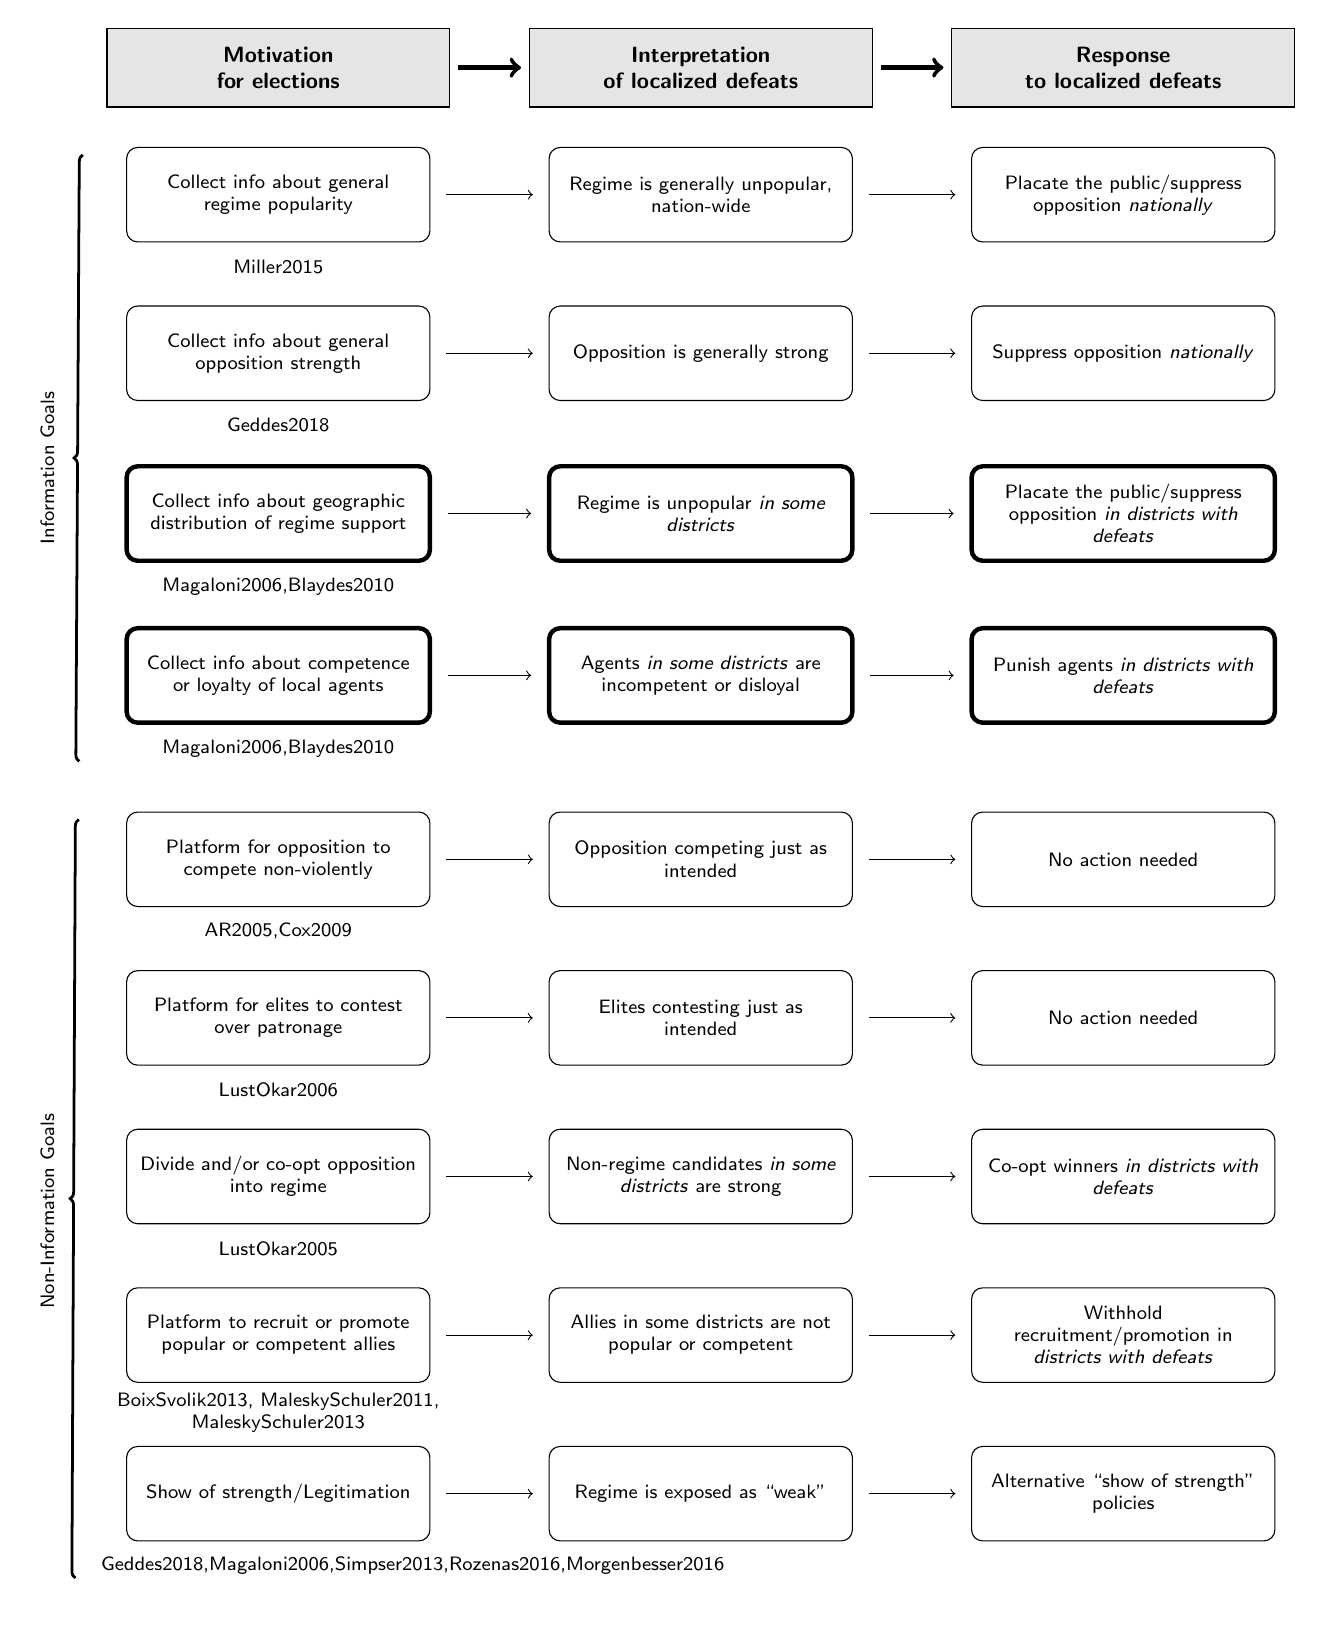
\begin{tikzpicture}
[node distance = 1cm, auto,font=\footnotesize,
% STYLES
every node/.style={node distance=3cm},
% The title style is used to draw the main title
title/.style={rectangle, draw, fill=black!10, inner sep=5pt, text width=4cm, text badly centered, minimum height=1cm, font=\bfseries\footnotesize\sffamily},
% The subtitle style is used to draw the title below main title
subtitle/.style={rectangle, inner sep= 2pt, minimum height=.5cm, node distance=0.25cm, text width=4.5cm, text badly centered, font=\scriptsize\sffamily},
% The theory style is used to draw nodes for each theory
theory/.style={rectangle, rounded corners, draw, minimum height=1.2cm, inner sep= 5pt, text width=3.5cm, node distance=0.25cm, text badly centered, font=\scriptsize\sffamily}]

%%%% Top nodes %%%%
\node [title] (interpretation) {Interpretation\\of localized defeats};
\node [title, left=1cm of interpretation] (intention) {Motivation\\for elections};
\node [title, right=1cm of interpretation] (response) {Response\\to localized defeats};

%% Top nodes subtitle

% Intention
%\node [subtitle, below=0.2cm of intention] (sub-intention) {for\\
%	authoritarian elections};

% Interpretation
%\node [subtitle, below=0.2cm of interpretation] (sub-interpretation) {of\\
%	localized defeats};

% Response
%\node [subtitle, below=0.2cm of response] (sub-response) {to\\
%	localized defeats};

%%%% Theory nodes %%%%
% B1
\node [theory, below=0.5cm of intention] (B1-intention) {Collect info about general regime popularity};
\node [subtitle, below=0.05cm of B1-intention] (B1-sub-intention) {\citep{Miller2015}};

\node [theory, below=0.5cm of interpretation] (B1-interpretation) {Regime is generally unpopular, nation-wide};
\node [subtitle, below=0.05cm of B1-interpretation] (B1-sub-interpretation) {};

\node [theory, below=0.5cm of response] (B1-response) {Placate the public/suppress opposition \textsl{nationally}};
\node [subtitle, below=0.05cm of B1-response] (B1-sub-response) {};

% B2
\node [theory, below=0.8cm of B1-intention] (B2-intention) {Collect info about general opposition strength};
\node [subtitle, below=0.05cm of B2-intention] (B2-sub-intention) {\citep{Geddes2018}};

\node [theory, below=0.8cm of B1-interpretation] (B2-interpretation) {Opposition is generally strong};
\node [subtitle, below=0.05cm of B2-interpretation] (B2-sub-interpretation) {};

\node [theory, below=0.8cm of B1-response] (B2-response) {Suppress opposition \textsl{nationally}};
\node [subtitle, below=0.05cm of B2-response] (B2-sub-response) {};

% B3
\node [theory, below=0.8cm of B2-intention, ultra thick] (B3-intention) {Collect info about geographic distribution of regime support};
\node [subtitle, below=0.05cm of B3-intention] (B3-sub-intention) {\citep{Magaloni2006,Blaydes2010}};

\node [theory, below=0.8cm of B2-interpretation, ultra thick] (B3-interpretation) {Regime is unpopular \textsl{in some districts}};
\node [subtitle, below=0.05cm of B3-interpretation] (B3-sub-interpretation) {};

\node [theory, below=0.8cm of B2-response, ultra thick] (B3-response) {Placate the public/suppress opposition \textsl{in districts with defeats}};
\node [subtitle, below=0.05cm of B3-response] (B3-sub-response) {};

% B4
\node [theory, below=0.8cm of B3-intention, ultra thick] (B4-intention) {Collect info about competence or loyalty of local agents};
\node [subtitle, below=0.05cm of B4-intention] (B4-sub-intention) {\citep{Magaloni2006,Blaydes2010}};

\node [theory, below=0.8cm of B3-interpretation, ultra thick] (B4-interpretation) {Agents \textsl{in some districts} are incompetent or disloyal};
\node [subtitle, below=0.05cm of B4-interpretation] (B4-sub-interpretation) {};

\node [theory, below=0.8cm of B3-response, ultra thick] (B4-response) {Punish agents \textsl{in districts with defeats}};
\node [subtitle, below=0.05cm of B4-response] (B4-sub-response) {};

% A1
\node [theory, below=1.1cm of B4-intention] (A1-intention) {Platform for opposition to compete non-violently};
\node [subtitle, below=0.05cm of A1-intention] (A1-sub-intention) {\citep{AR2005,Cox2009}};

\node [theory, below=1.1cm of B4-interpretation] (A1-interpretation) {Opposition competing just as intended};
\node [subtitle, below=0.05cm of A1-interpretation] (A1-sub-interpretation) {};

\node [theory, below=1.1cm of B4-response] (A1-response) {No action needed};
\node [subtitle, below=0.05cm of A1-response] (A1-sub-response) {};

% A2
\node [theory, below=0.8cm of A1-intention] (A2-intention) {Platform for elites to contest over patronage};
\node [subtitle, below=0.05cm of A2-intention] (A2-sub-intention) {\citep{LustOkar2006}};

\node [theory, below=0.8cm of A1-interpretation] (A2-interpretation) {Elites contesting just as intended};
\node [subtitle, below=0.05cm of A2-interpretation] (A2-sub-interpretation) {};

\node [theory, below=0.8cm of A1-response] (A2-response) {No action needed};
\node [subtitle, below=0.05cm of A2-response] (A2-sub-response) {};

% C1
\node [theory, below=0.8cm of A2-intention] (C1-intention) {Divide and/or co-opt opposition into regime};
\node [subtitle, below=0.05cm of C1-intention] (C1-sub-intention) {\citep{LustOkar2005}};

\node [theory, below=0.8cm of A2-interpretation] (C1-interpretation) {Non-regime candidates \textsl{in some districts} are strong};
\node [subtitle, below=0.05cm of C1-interpretation] (C1-sub-interpretation) {};

\node [theory, below=0.8cm of A2-response] (C1-response) {Co-opt winners \textsl{in districts with defeats}};
\node [subtitle, below=0.05cm of C1-response] (C1-sub-response) {};

% C2
\node [theory, below=0.8cm of C1-intention] (C2-intention) {Platform to recruit or promote popular or competent allies};
\node [subtitle, below=0.05cm of C2-intention] (C2-sub-intention) {\citep{BoixSvolik2013, MaleskySchuler2011, MaleskySchuler2013}};

\node [theory, below=0.8cm of C1-interpretation] (C2-interpretation) {Allies in some districts are not popular or competent};
\node [subtitle, below=0.05cm of C2-interpretation] (C2-sub-interpretation) {};

\node [theory, below=0.8cm of C1-response] (C2-response) {Withhold recruitment/promotion in \textit{districts with defeats}};
\node [subtitle, below=0.05cm of C2-response] (C2-sub-response) {};

% D1
\node [theory, below=0.8cm of C2-intention] (D1-intention) {Show of strength/Legitimation};
\node [subtitle, below=0.05cm of D1-intention] (D1-sub-intention) {\citep{Geddes2018,Magaloni2006,Simpser2013,Rozenas2016,Morgenbesser2016}};

\node [theory, below=0.8cm of C2-interpretation] (D1-interpretation) {Regime is exposed as ``weak''};
\node [subtitle, below=0.05cm of D1-interpretation] (D1-sub-interpretation) {};

\node [theory, below=0.8cm of C2-response] (D1-response) {Alternative ``show of strength'' policies};
\node [subtitle, below=0.05cm of D1-response] (D1-sub-response) {};

%%%% Side theory category nodes %%%%

% B
\node [subtitle, left=1cm of B1-intention.north west, rotate=90, text width = 8cm] (information) {Information Goals};

\draw [decorate,decoration=brace, line width=1pt] 
([xshift=-0.2cm, yshift=0.1cm]B4-sub-intention.south west) -- ([xshift=-0.55cm, yshift=-0.1cm]B1-intention.north west);

% A, C and D together
\node [subtitle, left=1cm of A1-intention.north west, rotate=90, text width = 10cm] (non-information) {Non-Information Goals};

\draw [decorate,decoration=brace, line width=1pt] 
([xshift=-0.25cm, yshift=0.1cm]D1-sub-intention.south west) -- ([xshift=-0.6cm, yshift=-0.1cm]A1-intention.north west);

%% A
%\node [subtitle, left=0.6cm of A1-intention.north west, rotate=90, text width = 4.4cm] (power-sharing) {``Platform''/``Power-sharing''};
%
%\draw [decorate,decoration=brace, line width=1pt] 
%([xshift=-0.2cm, yshift=0.1cm]A2-sub-intention.south west) -- ([xshift=-0.2cm, yshift=-0.1cm]A1-intention.north west);
%
%% C
%\node [subtitle, left=0.6cm of C1-intention.north west, rotate=90, text width = 1.9cm] (co-optation) {``Co-optation''};
%
%\draw [decorate,decoration=brace, line width=1pt] 
%([xshift=-0.2cm, yshift=0.1cm]C2-sub-intention.south west) -- ([xshift=-0.2cm, yshift=-0.1cm]C1-intention.north west);
%
%% D
%\node [subtitle, left=0.6cm of D1-intention.north west, rotate=90, text width = 2cm] (show-of-strength) {``Demonstration''};
%
%\draw [decorate,decoration=brace, line width=1pt] 
%([xshift=-0.2cm, yshift=0.1cm]D1-sub-intention.south west) -- ([xshift=-0.2cm, yshift=-0.1cm]D1-intention.north west);


%%%%%%%%%%%%%%%%

% Draw the links between forces
\path[->,ultra thick, shorten >=.1cm, shorten <=.1cm] 
(intention) edge (interpretation)
(interpretation) edge (response);

\path[->, shorten >=.2cm, shorten <=.2cm] 
(A1-intention) edge (A1-interpretation)
(A1-interpretation) edge (A1-response);

\path[->, shorten >=.2cm, shorten <=.2cm] 
(A2-intention) edge (A2-interpretation)
(A2-interpretation) edge (A2-response);

\path[->, shorten >=.2cm, shorten <=.2cm] 
(B1-intention) edge (B1-interpretation)
(B1-interpretation) edge (B1-response);

\path[->, shorten >=.2cm, shorten <=.2cm] 
(B2-intention) edge (B2-interpretation)
(B2-interpretation) edge (B2-response);

\path[->, shorten >=.2cm, shorten <=.2cm] 
(B3-intention) edge (B3-interpretation)
(B3-interpretation) edge (B3-response);

\path[->, shorten >=.2cm, shorten <=.2cm] 
(B4-intention) edge (B4-interpretation)
(B4-interpretation) edge (B4-response);

\path[->, shorten >=.2cm, shorten <=.2cm] 
(C1-intention) edge (C1-interpretation)
(C1-interpretation) edge (C1-response);

\path[->, shorten >=.2cm, shorten <=.2cm] 
(C2-intention) edge (C2-interpretation)
(C2-interpretation) edge (C2-response);

\path[->, shorten >=.2cm, shorten <=.2cm] 
(D1-intention) edge (D1-interpretation)
(D1-interpretation) edge (D1-response);


\end{tikzpicture} 
\caption{Key theories of authoritarian elections and their predictions about how regime leaders perceive and respond to localized defeats. Two theories most relevant to the Vietnam case are highlighted with bold borders.}
\label{fig:Theory}
\end{figure}


\section{Identify the Purpose of Vietnam's Elections}
\label{sec:vietnam}

In the above sections, I argued that authoritarian regimes are judicious in deciding what they want their elections to achieve, such that they should prioritize only a subset of goals when holding elections. I also suggested that, among those goals pertaining information collection, studying these regimes' responses to the defeats of their candidates in parliamentary elections may identify exactly which goals they prioritize and thus which kind of information they need. In this section, I demonstrate this logic by looking at the Vietnamese government's response to a certain kind of election defeats, and show that, given the constraints of a highly institutionalized single-party regime, regime leaders in Vietnam choose to use elections to gather information on the distribution of support it has across sub-national units. 

Vietnam is an ideal case because it is a single party regime whose leaders are able to exercise near-perfect control over election results, yet intentionally refrain from completely manipulate the entire electoral process \citep{MaleskySchuler2011}, suggesting that they may indeed be using elections for some purposes. A close look at the structure of authoritarian rules in Vietnam suggests two informational needs that elections could potentially fulfill, but is not sufficient to determine which of them is actually serviced by elections. An empirical treatment using unexpected local defeats is thus expected to be very useful in this case.

\subsection{Two Authoritarian Information Problems in Vietnam}
\label{sec:vietnam_problems}

\subsubsection{Information about distribution of regime support}

As a single-party state ruled by a strong Communist party, Vietnam is a representative case for most theories about institutionalized single-party states. Formally, Vietnam has a parliamentary system with a popularly elected national legislature, which in turn elect the executive. In practice, however, the ruling Communist Party of Vietnam (CPV) controls the entire political system, including membership in both the legislature and in the executive branch; the CPV also maintains a party bureaucracy that intertwines with the administrative bureaucracy at all levels of government. 

Like in most authoritarian regimes, the CPV leaders face the ``Dictator's Dilemma'' \citep{Wintrobe2000}: even as the regime needs to ascertain its popularity among the public, it also has to prevent people from expressing dissatisfaction through the threat of punishment, which then discourages the public from revealing their true preference for the regime. Generally, however, the CPV can rest assured that its general \textit{level} of support is sufficiently high: the party benefits from a long historical legacy as the revolutionary party that had brought independence from the French in 1945 and unified the country after the Vietnam War in 1975, a recent periods of high economic growth, as well as tight control over the media and other propaganda apparatus that neutralize most attempt to tarnish its image. Indeed, results from the World Values Survey \citeyearpar{wvs} and the Asian Barometer \citeyearpar{abs} have consistently indicate very high levels of confidence in the government.\footnote{Specifically, Wave 5 of the World Values Survey \citeyearpar{wvs} found that 77.8\% of respondents have ``a great deal'' and 17.9\% have ``quite a lot'' of confidence in the government, and Wave 3 of the Asian Barometer \citeyearpar{abs} found that 85\% of respondents either ``strongly agree'' or ``agree'' that they trust government officials.}

Governing over a population of more than 90 million people and a territory spanning more than 15 degrees latitude, however, the CPV cannot be confident that its popularity is evenly \textit{distributed} across the country. Although moments of unrest such as protests or riots are extremely rare, they have emerged from isolated pockets of dissatisfaction, such as in Binh Thuan in 2018, Ha Noi in 2017, or Ha Tinh in 2016. In addition, some regions such as the Central Highlands, home to a large ethnic minorities population, also pose some non-trivial security threats. As a result, even as the CPV know that it enjoys a high level of popularity, it still needs to worry about the potential of deteriorating support in smaller sub-national units. 

Information about this, however, is largely unavailable. Not only are international surveys such as the World Values Survey or Asian Barometer not covering enough respondents for sub-national aggregates to be reliable, but the regime's own attempts at studying public opinion in these provinces are also inadequate.\footnote{According to my interview with an official in the Party's public opinion research unit, the Party does not conduct large-scale surveys that can be quantitatively analyzed. Instead, it relies primarily on networks of grassroot informants whose reports do not allow for effective cross-region comparisons.} In addition, the regime's other authoritarian institutions also fail to provide reliable insights: the media is largely muted by tight control, whereas reporting by local government officials are likely subjected to intentional embellishment, because these officials are also evaluated for promotion based on their ability to maintain low levels of dissent.

On the other hand, the CPV does relatively well in securing most other types of information. For example, it has little additional needs for information on opposition strength or potential dissidents other than those already secured by the large security apparatus. By keeping close watch over social media, the regime also learns quickly which political or social issues are attracting public attention as well as general opinion on these issues, allowing it to react quickly. 

\subsubsection{Information about regime agents}

There is, however, one other informational concern that regime leaders in Vietnam have not successfully addressed. In particular, the CPV has particular needs for information on its own rank-and-file members, in particular their competence and loyalty. As a highly institutionalized party that controls all branches of government, the CPV depends on a large number of bureaucrats and party agents to govern; it also needs to provide meritocratic promotions pathway to encourage performance and loyalty from these subordinates \citep{Svolik2012}, and does so through a cadre management system not different from China's \citep{Manion1985}. For this system to function, however, the party needs to be able to identify high-performing bureaucrats to promote, which then requires discerning their ability from external factors. In addition, the central leadership in Hanoi also needs their agents to devote more loyalty to it than to local power brokers in the periphery. In particular, although many of the top officials in its 63 provinces are outsiders appointed by the central leadership, day-to-day government affairs at lower levels are conducted by bureaucrats who are often native to the locality they serve in.\footnote{The distinction between two types of government agents is closely linked to the distinction between ``deployed'' and ``delegated'' bureaucrats made by \cite{Soifer2015} in his study of state-building in Latin America} Without monitoring, even these top officials may collude with local bureaucrats to implement policies in ways that serve their interests instead of the center's.

Information about competence and loyalty of party officials and bureaucrats is important because these agents both directly impact the party's governance performance and indirectly influence the public's perception of the party at the local level. Through extensive reporting requirements, the CPV's leadership has access to a large array of indicators that would allow them to assess both these variables. However, two factors reduce the utility of this information. First, these outcome- and output-based measures do not account for variation in external factors that make achievements inherently incomparable across sub-national units. For example, achieving a high growth rate is much easier for port cities than highland provinces. Secondly, sub-national officials have both the incentive and the capacity to misreport the very indicators they are evaluated on, which calls into question their usefulness as benchmarks for both competence and loyalty. For these reasons, the CPV still has dire needs for reliable and standardized information about its own agents. As the next sections will show, however, when it comes to deciding which information to collect with elections, Vietnam's regime leaders still prefer to learn about the sub-national distribution of support for the regime rather than about the quality of its officials.  

\subsection{Which Information Problem Do VNA Elections Solve?}
\label{sec:vietnam_solutions}

\subsubsection{Authoritarian Elections in Vietnam}
\label{sec:vietnam_elections}

The elections for the Vietnamese National Assembly (VNA) are representative of tightly-controlled parliamentary elections under secure authoritarian regimes. Details of the nomination and election process for these elections have been thoroughly explored by \cite{MaleskySchuler2011}, among others \citep[e.g][]{Gainsborough2005}, some of which are particularly important. Specifically, the VNA elections follow an absolute-majority voting system with multiple winners, in which each district can have 3 to 6 candidates running for 2 to 4 seats and voters get to vote for as many candidates as there are seats in the district. District magnitude and number of candidates are determined prior to the election based on population sizes, and follow a fixed formula: a 6-candidate district is allowed 4 seats, a 5-candidate district is allowed 3 seats, and a 4-candidate district is allowed 2 seats.\footnote{A new type of district with 3 candidates with 2 allowed seats was introduced for the 2011 election, but were then discontinued by the 2016 election.} Because voters cast multiple votes, the vote share total in each district can range from 200 to 400 percent, but each candidate can secure 100 percent at most. In all districts, candidates with the most votes win, as long as their number of votes exceeds 50 percent of registered voters. This form of voting obscures the informational value of vote margins, as one candidate's margin over another also depends on the performance of that other candidate \textit{vis-\`{a}-vis} another.

The key dynamics of these elections, however, take place not on election day, but in the nomination process that precedes it. In this process, before each election, the central party leadership in the outgoing VNA, which is organized as the VNA standing committee (VNASC), draws up a structure for what the incoming NA should look like. The structure takes the form of composition along demographic, political, and functional lines; for instance, the planned structure for the 500-delegate VNA in the 2007 election called for 150 women, 90 members of ethnic minorities, 160 incumbents, 70 under-40 delegates, and 50 non-party members  \citep[506]{MaleskySchuler2011}. Then, through three rounds of \textit{hiệp thương} (negotiation), the central party leadership and provincial institutions put together a list of candidates to fill the slots, and assign them to districts in ways that would best guarantee that the elected VNA follows the planned structure. This is done by first determining quotas breaking down how many candidates of a certain demographic each province (and then each district) should elect, and then ``stuff'' the districts with candidates from this same demographic. For instance, a district the regime expects to elect a lawyer would be contested only by lawyers, a district it expects to elect a member from an ethnic minority would include only candidates from ethnic minorities, etc. As a result, even though within a district individual candidates may compete against each other to gain votes, the aggregate structure of the VNA can be guaranteed. Additionally, even when the CPV allows independent and self-nominated candidates to contest elections, the nomination process also acts a filter to ensure that only those who follow closely the party line are allowed to run.

A central feature of this nomination process is the difference between central and local nominees. Central nominees are candidates who are nominated in the three \textit{hiệp thương} rounds by central party and government institutions, as well as by the national bodies of party front mass organizations. In practice these central nominees are high-ranking party members with important roles in the party or the government, current VNA committee members, or national leaders of these mass organizations. Local nominees, on the other hand, are nominated by provincial level party and government branches as well as by local chapters of the same organizations. During the \textit{hiệp thương} rounds, central candidates are assigned to individual districts, where they will run against local nominees coming from the local province. Central nominees comprise roughly a third of the planned VNA structure, and all of them are expected to win seats. According to \cite{MaleskySchuler2011}, the CPV ensures this outcome by tilting the playing field \textit{ex ante} rather than through election-day manipulation. In particular, they assign these central nominees not to their home districts or districts they have previously served, but to districts where they can win more easily i.e. districts with the more favorable 5-to-3 candidate-to-seat ratio. In addition,  central nominees generally are not assigned to run against each other. Finally, provincial officials are instructed to support these candidates, both by nominating and assigning  weaker candidates to run against them, as well as by running voter education and mobilization campaigns to encourage voters to vote for them. 

\subsubsection{Information about distribution of regime support}

As argued in section \ref{sec:theory_priority}, authoritarian regimes can optimize the informational values of elections through selective use of election manipulation tactics. There are good reasons to believe that the VNA elections in Vietnam are optimized with public opinion collection in mind. First of all, the high level of control the CPV has over election outcomes keeps local defeats rare but not impossible, such that any defeat that does happen is more likely to be signal than noise. Indeed as \cite{MaleskySchuler2011} show, the party is confident enough in its ability to control election results to set out very specific plans for the structure of the to-be-elected VNA, and the near-identity between planned and the actually elected VNA shows that its confidence is well warranted. However, the fact that the final result detracts slightly from the plan suggests that the CPV's control is not perfect. Indeed, in all three most recent elections, there have always been central nominees who suffered unexpected defeats, even though they never comprised more than 15 percent of all the running central nominees: 21 out of 165 for 2007, 14 out of 173 for 2011, and 16 out of 197 for 2016. Their defeats were surprising and important enough to be covered by the state-controlled media \citep[e.g][]{vov2016, laodong2016}. At the same time, the lack of perfect control over election outcomes do not seem unintentional: \cite{MaleskySchuler2011} show that the CPV does not engage in outright forms of manipulation such as tampering with vote tallies or ballot stuffing.\footnote{\cite{MaleskySchuler2011} arrived at this conclusion after conducting digit tests on official results from the 2007 election fail to reject the hypothesis of naturally generated numbers. In Appendix \ref{app:benford} I replicate the same findings for the 2011 and 2016 elections. However, this evidence would only rule out fraud at the highest level but fail to detect manipulation at lower level, as aggregates of manipulated numbers would exhibit patterns similar to the natural generation process. Indeed, interviews with neighborhood-level officials in charge of managing the 2016 election suggest that agents at several polling stations tampered with the tabulation of result. There is however no smoking-gun evidence that such tampering is systematic or ordered by higher levels of government.} Given that this kind of manipulation would reduce the informational value of election results, there are reasons to believe that the CPV is truly seeking something from these results other than overwhelming victories.

Secondly, the CPV's other electioneering strategies could be seen as attempts to not only increase control over election outcomes but also refine the range of potential factors that could determine any particular set of results. Specifically, by assigning many of the central nominees to provinces they are strangers in, the central leadership could ensure that election results are not driven by these candidates' popularity among their constituencies. Similarly, because outsiders are prevented from running, voters have no opportunity to signal support for regime opponents, which rule out opposition support as a determinant of the final tallies. 

Thirdly, the massive mobilization campaign conducted prior to each election has the effect of associating central nominees with the party itself, such that voters see voting against these nominees as casting a vote of no confidence against the central government. Indeed, as part of this campaign, neighborhood-level officials visit individual households to inform voters of the candidates' profiles, as well as conveying ``suggestions'' about which candidates to vote for. Since these suggested candidates are already strangers -- in contrast with local nominees, who most likely would have spent their entire careers in the province -- voters are guaranteed to have plenty of cues, if not about which candidates are central nominees, then about which candidates the government truly prefers. In light of this, it is not inconceivable that voters can associate voting against central nominees with expressing dissatisfaction against the central government.

Although the above cannot be directly verified, but my interviews both formal and informal with voters in Hanoi and Ho Chi Minh City suggest that a number of them do exhibit exactly this kind of behavior. In particular, some voters comment that they crossed out the names of whoever the neighborhood official suggests to them, whereas some others voted only for independent candidates. In this sense, the door-to-door voter education actually emphasized the link between central nominees and the central government, thus providing voters with targets to direct their disapproval. Furthermore, interviews suggest that voters in Vietnam have high confidence that their ballots are kept secret, but also low confidence that they are tabulated correctly. These two beliefs are not contradictory: on the contrary, voters think their ballots are kept secret \textit{precisely because} they believe the regime will not even look at them, choosing instead to make up results in the tabulation process. This means that some voters see voting as an inconsequential act of expression, and do so freely without fear of retribution when dissatisfied. In the end, these voters may have underestimated their efficacy: where voters cast more of such ``protest votes,'' central nominees may end up losing elections despite the biases in their favor.

Thanks to these design features of the VNA elections, when local defeats did indeed occur, the space of possible explanations are already limited enough that the CPV can interpret these defeats as indicators for provinces where support for the CPV has reached an alarmingly low level. Since elections take place in the entire country and on the same date, the information from them are both comparable and standardized, which helps enhance its quality. In this sense, the VNA elections serve as a reliable public opinion census for the CPV.

If the CPV was indeed using the VNA elections to identify which provinces it is less popular in, it would join a large number of other authoritarian regimes who have been documented to do the same thing. In Mexico for example, \cite{Magaloni2006} finds that the PRI deemed areas where they captured a greater vote share were deemed as centers of government support, whereas areas with low PRI vote shares were considered opposition strongholds. Similarly, for Egypt, \cite{Blaydes2008} remarks that ``election results provide the regime with a map of areas of political support for the opposition.'' In both cases, the two authoritarian governments were able to know which sub-national units have higher or lower concentration of regime supporters by looking at where they received a higher or lower vote share. In Vietnam, elections could have served an identical role.

\subsubsection{Information about regime agents}

At the same time, however, certain other features of the VNA elections also raise the possibility that the CPV designs these elections as a standardized measure of regime agents' performance, an information it also sorely needs. In particular, the delegation of election management to provincial officials leave open the possibility that these officials could influence the final results. In this light, local defeats could reveal important information about the competence and loyalty of provincial leaders. 

To understand why election results reveal information about provincial officials, it is important to understand the extent to which these officials can influence election results. First of all, provincial leaders reserve the freedom to nominate local candidates in their provinces and allocate these candidates to electoral districts. Provincial leaders can therefore reduce competition for central nominees by stacking them up against weaker local candidates, or by placing them in districts with more favorable candidate-to-seat ratios. This indeed is a common practice \cite[provided confirmatory evidence for the 2007 election, which I replicated successfully for the 2011 and 2016 elections]{MaleskySchuler2011}.  Additionally, through the infrastructure of the state, local officials can have significant power to directly influence the voters' choices. The door-to-door voter education and mobilization campaign carried out at every neighborhood is a example. If the majority of voters are passive and/or apathetic compliers -- instead of active ``protest voters'' as described above -- then provincial officials can definitely influence election results just by selecting who they tell voters to vote for. Finally, provincial officials can also interfere with the tabulation of results such that the candidates they prefer receive favorable vote shares regardless, even when such local-level manipulation may not be in the best interest of the central government. 

However, it is not entirely in these provincial officials' interest to fully exercise their power in support of central nominees. This is because the provinces also have vested interest in ensuring as many of their candidates as possible make it to the VNA, since these local nominees are either local leaders in the provinces, or representatives of local interests. Although top provincial leaders are appointed by the central government and are often not native to the province they work in, the long tenure of 4-5 years makes it attractive for them to align with the province's interests. Center-periphery divide arises because each elected central nominee takes one seat away from local candidates. Indeed, in 2016, the municipality of Hanoi reportedly demands to have fewer centrally nominated candidates to make room for its own candidates \citep{vnexpress2016_2}. Occasionally, strong central nominees can cost the province even more than one seat. In particular, when central candidates secure too many of the district's votes, the chance that some local candidates may not make it pass the 50 percent threshold increases. When this happens, the district may not be able to elect as many candidates as there are seats allotted for them -- as happened in two provinces in 2016 \citep{vnexpress2016}. As consequence, even when the central party leadership expects provincial officials to deliver election results that follow the planned structure and that give seats to all central nominees, any province that does this too enthusiastically may end up costing itself a representative in the VNA. This means that local officials operate within the boundary of divergent preferences: while the center prefers provinces to devote as much resource as \textit{possible} to the promotion of central nominees, provincial leaders only seek to do so as much as \textit{necessary} to avoid hurting their own candidates. In the ideal scenario, this produces a result acceptable to the center, but when the local officials are too eager to support their own candidates, or too incompetent to exercise their power effectively, central nominees are at risk of losing to local candidates.

The fact that Vietnam's central government allows province-level officials to have such influence over election outcomes raises the question of whether it does so out of an efficiency consideration, or as a way to gather information about these officials. On one hand, the latter hypothesis seems plausible when considering how the deliver of votes for central nominees in a national election provides a comparable yardstick for provincial officials' competence and loyalty -- a ``standardized test'' that the CPV truly needs. Indeed, authoritarian rulers have made use of the same tactic in some other contexts, such as Egypt \citep{Blaydes2008}, or Mexico \citep{Magaloni2006, Larreguy2016}. On the other hand, interpreting local defeats as signals about regime agents' performance interferes with these defeats' value as indicators for provinces with low levels of government support. Indeed, as section \ref{sec:theory_priority} argues, intending for the VNA elections to gather both types of information would only prevent effective learning on the part of the CPV. It is therefore expected that, despite both being plausibly generated from the VNA elections, only one of these two information was being intentionally sought by the CPV.


\subsection{How Post-election Responses Answer This Question}
\label{sec:vietnam_responses}

In reality, pockets of low government support \textit{alone} or slacking provincial officials \textit{alone} are unlikely to be responsible for central nominee defeats in the VNA elections. Indeed, the true cause is most likely a combination of both these factors as well as other unforeseen variables. In the eyes of the Vietnamese regime, however, only one interpretation can be accepted -- one that sheds light on the information it originally seeks from these elections. This is because interpreting central nominee defeats as product of multiple causes introduces the difficult problem of assigning weights between these causes, which leaves the CPV uncertain about which lesson to draw from these defeats. Furthermore, the institutional setting in Vietnam is such that the CPV can only acts on one of the two interpretations at once. 

Specifically, if the regime has intended to use the VNA elections to gather information about the distribution of public opinion, it would interpret local defeats as indicators for provinces with faltering public support. For the CPV, the appropriate post-election response would be to  \textit{increase} central transfers to these provinces to \textit{placate} the public. In Vietnam, because most provinces spend more money than it can generate through taxes, central transfers are indispensable for public goods provision. Increasing central transfers thus enables increased spending on public goods and other popular programs, which is the most straightforward way to bolster support for the regime. In some ways, this outcome leads to partial fulfillment of \textit{bottom-up accountability}, in which citizens hold government accountable for the provision of public goods through their votes.

Note that not every authoritarian regime is expected to increase financial support to areas it identifies as low-support. Indeed, as \cite{Magaloni2006} and \cite{Blaydes2008} find in their studies of Mexico and Egypt, the opposite happen: the regime punishes provinces with lower party vote share by cutting central transfers to these provinces. The reason a placation strategy seems reasonable in Vietnam but not in Mexico or Egypt is because the level of competition is different. In Vietnam, there is no organized opposition, and so a low vote share would only reflect dissatisfaction towards the CPV, not affinity to any particular opposition party. In addition, the general level of support for (or at least ambivalence about) the party is still high, with very few people who could be counted as dissidents. In this context, a sweeping ``punishment regime'' \citep{Magaloni2006} would hurt regime supporters more than it would punish dissidents. A  placation strategy, on the other hand, would soothe dissatisfaction without incurring resentment.\footnote{A possible concern is that this strategy would create perverse incentive for voters to vote against the regime in future elections. In Vietnam, however, the CPV could avoid this by not publicly drawing connection between public finance policy and election results. Since elections happen only every 5-6 years, it will not be easy for voters to notice that voting down central nominees can increase central transfers to their provinces. Additionally, discussions about budget decisions are kept confidential from the public.} Indeed, this logic is consistent with cross-national evidence that authoritarian regimes increase spending on public goods in response to weak electoral performance \citep{Miller2015}, and with the argument from the clientelism literature that patronage money serves authoritarian leaders best when it flows to ``swing voters'' \citep{DixitLondregan1996, Stokes2013}.\footnote{Empirically, this literature, in particular \cite{Stokes2013}, finds that patronage often flows instead to ``core voters'' who are already voting for the ruling party and whose voting behavior is not impacted by patronage money. This seemingly inefficient distribution of clientelistic benefits arises from principal-agent conflict between the party machine and the low-level brokers who are tasked with the actual distribution of these resources. In the context of central transfers in a centralized regime like Vietnam, however, there is no need for brokers to mediate between the central government and individual provinces. Finally, even in the presence of brokers, \cite{Stokes2013} still finds that clientelistic flows to swing \textit{districts} even as it flows to core \textit{voters} within these districts. As a result, if the analogy between post-election central transfers and clientelism is to be accepted, we can expect central transfers in Vietnam to still flow to swing districts i.e. provinces that suffered local defeats.} 

On the other hand, if the CPV uses the VNA elections to evaluate its province-level agents, it would see from central nominee defeats the identity of provincial leaders who are either incompetent or disloyal. The logical reaction would then be the opposite, namely the CPV would seek to \textit{decrease} central transfers to provinces with local defeats in order to \textit{punish} the agents tasked with managing elections there. Cutting central transfers is the most effective option for punishment since it directly affects the officials' income by reducing their opportunity to engage in corruption, particularly graft. In a tightly controlled authoritarian regime like Vietnam, corruption is often allowed as a means for the central government to compensate lower level officials \citep{Darden2008}. For these local officials, not only is graft an important source of income, but the ability to distribute rent further downwards is also the source of their political power.\footnote{An implication of this argument is that the election of central nominees at the expense of local nominees can be a negotiated outcome: provinces that are more powerful vis-\`{a}-vis the central government may be able to push for the election of their own nominees and accept the punishment as the cost of doing so. Indeed, \cite{MaleskySchuler2011} find that central nominee defeats are more likely in provinces that depend less on central transfers.} (To confirm this intuition, in section \ref{sec:results} I show that other popular punishment methods are not employed in response to election results.)

A possible concern is that cutting transfers may reduce the resources available to local bureaucrats, making it harder for them to successfully deliver the next election. This makes the next election's results less informative, since defeats could now happen despite the province's best efforts. In the Vietnam case, however, this concern can be left to rest. Firstly, provinces in Vietnam receive dedicated funding for election management during election years. Secondly, provincial officials often get promoted or moved to a different province just before the election. Together, these two characteristics of the Vietnam means that public finance punishment in one election would not handicap or advantage individual bureaucrats in the next.

The cycle of leadership overhaul in Vietnam also rules out withholding promotion as a method of punishment, which has been used in other nondemocratic regimes such as Russia \citep[][136]{Myagkov2009}. In particular, the major overhaul of leadership positions in Vietnam only happens around election years, and always takes place shortly before the election.\footnote{More precisely, both leadership overhaul and legislative elections are scheduled to coincide with the National Party Congress, which happens every five years. During the Party Congress, the CPV's top leaders and delegates from all over the country meet to decide on the party's leadership for next five-year term. The Congress decides who would fill the top three leadership positions -- Prime Minister, President and General Secretary of the CPV -- and consider the promotion of lower level party members into higher positions within the party hierarchy. All provincial officials, as well as most central nominees for the legislative election, are then drawn from this pool of high-level party officials.} An official therefore will not experience the impact of promotion withholding until the next election, thus rendering the efficacy of this method as a punishment much lower. Additionally, demotion or firing is almost never an option except for very serious transgressions, possibly because such punishment would shatter the image of infallibility that the regime tries to create and draw attention to disunity within the party leadership.\footnote{Two illustrative anecdotes demonstrate the point that the CPV tries to avoid drawing attention to punishment decisions within the party, and that it only punishes top officials in case of extreme transgressions. Firstly, in 2012, when the CPV's highest leadership debated and decided against officially censuring then-PM Nguyen Tan Dung for economic mismanagement, official statements from the Party refers to him only as ``one comrade'' without mentioning any name \citep{voa2012}. Secondly, in 2017, when the Party's leaders finally decided to punish Ho Chi Minh City's Party Secretary Dinh La Thang and to publicly acknowledge this decision, it was only after mismanagement of PetroVietnam, Vietnam's largest SOE and where Thang had served as chairman between 2009 and 2001, has been found to cost the country close to US\$150 million \citep{BBC2017}.} Finally, promotion decision in Vietnam is already determined by other factors beyond election performance, such as FDI promotion \citep{JensenMalesky2018} or aggressive bargaining by individuals (as suggested by my qualitative interviews). As a result, cutting opportunity for graft through lowering central transfers remains as the most plausible punishment for local defeats, conditioning on the regime’s believing that election results are primarily determined by party bureaucrats. This logic of punishing lower-level party cadres for failing to perform a target set by national leadership can be said as describing \textit{top-down accountability}.

It is also worth noting that evidence of punishment through cutting central transfers should never be expected if the CPV was using elections to identify areas it lacks support in. Indeed, reducing transfer would render the regime even more unpopular because of this strategy's negative impact on public goods provision, hurting it in the next election. In this sense, if the CPV chose to cut central transfers to provinces it had suffered defeats, in must have firmly believed that its level of popularity there has little to do with election outcomes if not for the incompetence or disloyalty of local bureaucrats.

Given the contradiction in the two post-election courses of action, it is straightforward to use public finance outcomes to identify what Vietnamese regime leaders see in their authoritarian elections. In particular, by finding out whether central transfers to a province increase or decrease following the defeat of central nominees in that province, it is possible to know whether elections in Vietnam function as a source of information on the distribution of regime support or on individual party agents. The absence of an effect, on the other hand, would suggest elections serve neither of these two roles. In such case, the other roles of authoritarian elections in Figure \ref{fig:Theory} represent possible null hypotheses, ensuring that this paper's research design is falsifiable, and not a blind empirical test for which any result would pass as a finding.

% UP UNTIL HERE ON MARCH 09
\section{Data and Methods}
\label{sec:methods}

To demonstrate that the ruling party in Vietnam uses elections as a source of information on its distribution of support across the country, and accordingly responds to serious but localized electoral setbacks by financially placating the localities it suffered defeat it, I focus on post-election changes in central transfers from the CPV leadership in Hanoi to individual Vietnamese provinces following the recent 2016 VNA election. As previously argued, in the context of Vietnam, decisions about central transfers are highly indicative of the regime's intentions, such that an increase in transfers to provinces where the regime's preferred central nominees were defeated would signal a preference for elections to serve as indicator of local public support. On the other hand, a decrease in transfers to these provinces would suggest that the regime sees elections as providing information about the locality of local agents. Finally, any inconclusive result would rule out both purposes of authoritarian elections as inapplicable to Vietnam.

From a practical point of view, testing the two theories using central transfers decisions benefit from the availability of public finance data in Vietnam. Specifically, the amount of central transfers allocated to each province each year can be easily calculated from Vietnam's national budgets by subtracting a province's expenditures from its revenues. Annual national budgets in Vietnam are publicly available both as planned and realized budgets for every year from 2004 to 2018. For this paper, I calculate central transfers allocation to each province using planned budgets, since budget plans are arguably more reflective of the regime's intentions than realized numbers. In addition, I cross-reference these numbers against province-level budgets that are made sporadically available by provincial governments over the same period, which helps allay some concerns over the quality of data and statistics released by the CPV.

I focus particular on the 2016 election for two reasons. Substantively, the 2016 election is the first election under this current administration, one that came to power through a relatively unexpected and contentious series of events.\footnote{In Vietnam, the National Party Congresses, which take place every 4 to 5 year, are responsible for deciding the country's top leaders. Legislative elections are generally held a few months after these congresses, partly in order to legitimize appointment decisions made in the congresses. The 2016 National Party Congress saw unexpected tension, with the top leadership position competed by the incumbent Prime Minister Nguyen Tan Dung and the incumbent Party General Secretary Nguyen Phu Trong. Initially favored to win, Nguyen Tan Dung was eventually defeated some last-minute maneuvering by Nguyen Phu Trong and his allies, and was forced to retire. In the incoming administration, then-Deptuty Prime Minister Nguyen Xuan Phuc serves as Prime Minister, the public security general Tran Dai Quang serves as President, and Nguyen Phu Trong continues as the Party General Secretary. \url{https://www.nytimes.com/2016/01/19/world/asia/vietnam-communist-party-congress.html}} Because this was no smooth transition of power, it seems plausible that the new leadership would be in need of information to assess its hold to power, both about their popularity and about the quality of existing subordinates, many of whom have been appointed under the previous administration. 

Practically, the 2016 election is also unprecedented in terms of data availability: it is the first election for which results are released for all candidates: in previous elections, vote counts and shares are made available only for winners, which preclude most empirical strategies that seek to leverage the closeness of elections. By matching these results with public profiles of all the candidates (publicized several months before the election) and identify from those candidates that were nominated by central-level agencies and organizations, I am able to construct a candidate-level dataset, from which province-level treatment data can be derived.

Even with this data, adjudicating between the two theories using central transfers outcomes remain a difficult causal inference problem. Across Vietnam's 63 provinces, because local defeats are not exogenously assigned, those that suffered such defeats may be different from those that did not in ways that matter for central transfers, regardless of the outcomes. For example, \cite{MaleskySchuler2011} show that these provinces are more politically dependent, in the sense that they need less central transfers and are located mostly in the South. The very premise of this paper also suggests that these provinces may have less supportive voters or lower quality bureaucrats -- indeed, it is precisely to measure these differences that the CPV holds elections in the first place. At the candidate level, it is widely expected that some candidates are more likely to lose than others. Most clearly, no matter how much information the regime may want to learn from this election, it is not going to tolerate the Prime Minister or the Party Secretary losing and consequently being unable to hold posts in the government. To ensure these that these important candidates secure victories, the CPV may make them run in provinces they have greater control over, for example those that receive and thus depend more on central transfers.

In addition, the relationship between election results and central transfers may also exhibit dynamic causality \citep{ImaiKim2012} because central transfers in pre-election years (past outcomes) may influence both central transfers in post-election years (future outcomes) as well as election results (treatment). In particular, low central transfers in pre-election years do not just reflect peripheral independence as previously argued, but may also make it harder for the province to provide public goods or fund election mobilization efforts, both of which can play a role in making local defeats more likely.

Finally, because the tightly managed election makes local defeats extremely rare, statistical inference becomes particularly challenging. Specifically, the low number of treated cases means that statistical power is small and that real effects even if existent may not be detected. Furthermore, effects that end up being detected may simply represent extreme aberrations that occur by chance and do not reflect the true state of reality i.e. ``Type M'' errors according to \citet{Gelman2014}.

I take several steps to overcome this array of empirical challenges.  First of all, I restrict my analyses to only provinces where central candidates lost or won narrowly. Because most defeats are close, most of the dropped provinces are those competed only by powerful top leaders whose defeats are unlikely. The logic behind this approach closely resembles that behind matching: by dropping cases with practically zero chance of being treated I can arrive at a comparison group more similar to the treated group \citep{Hoetal2007Matching}. It is also similar to the local randomization logic of the regression-discontinuity design, which achieves causal identification by assuming that treatment is as-if random among treated units that are close to being in control and control units that are close to being treated \citep{CattaneoTitiunik2015}. I define close wins as cases where central candidates won with a margin of no more 10 percentage points to the closest losing local candidates, or with a vote share of no more than 60 percent.\footnote{The 60 percent threshold is officially considered a low winning threshold by the CPV – winning candidates with vote shares below it are required to formally self-criticize \citep{MaleskySchuler2011}.} I also drop from the sample the capital Ha Noi and the second biggest city Ho Chi Minh City since they are different from other provinces in almost every relevant dimension.\footnote{Together, the pruning restricts the data to observations that narrowly received treatments and their closest counterfactuals, meaning that the causal estimand arising from comparing these two groups can best be understood as the local average treatment effect (LATT). Since most defeats were close, however, the LATT is substantively similar to the ATT.}

Secondly, I leverage the panel structure of the data and employ linear fixed effects regressions to help reduce omitted variable bias. Specifically, I fit the following model to the pruned dataset:

\begin{equation}
\Delta Y_{it} = \beta D_{it} + \omega T_{i} + \gamma X_{it} + \lambda_i + \delta_t + \epsilon_{it} \label{eq:FE}
\end{equation}
where $\Delta Y_{it}$ is the log of the first difference in net central transfers for province $i$ at time $t$ i.e. $\Delta Y_{it} = \log(Y_{it} - Y_{i, t-1})$, $X_{it}$ is a vector of time-varying covariates, $D_{it}$ marks the treatment status for treated years and $T_{i}$ marks the treatment status for all the years. Specifically, $T_{i}$ takes the value of 1 for every province that experienced local defeat in 2017 and 0 otherwise, and does so for every year in the sample. On the other hand, depending on whether the model seeks to estimate the \textit{instantaneous} effect that occurs in the one year immediately after the election, or the \textit{persistent} effect that manifests in all post-election years, $D_{it}$ is equal to $T_{i}$ for $t=2017$ or $t\geq2017$, and is equal to $0$ otherwise.\footnote{The ``lagged'' treatment indicator accounts for the fact that budget allocation decisions are made at the beginning of each year, such that the effect of the 2016 election only begins to manifest in 2017.} Here, for arbitrary functions $h(\cdot)$ and $g(\cdot)$, $\lambda_i = h(\mathbf{U}_t)$ is the province fixed effects and $\delta_t = g(\mathbf{V}_t)$ is the time fixed effects, which together help zero out selection bias due to time-invariant confounders $\mathbf{U}_i$ and capture time-varying common shocks $\mathbf{V}_t$. For most analyses, $t \in \{2012, \cdots, 2018\}$ to exclude the years before the previous election.

To understand the use of first-differenced outcome in this model, Appendix \ref{app:proof1} shows how the model in \ref{eq:FE} is a generalized version of the triple differences (or ``difference in differences in differences'') framework, similar to how a typical linear fixed effects regression is a generalized version of the difference-in-differences framework. Generally speaking, the triple differences framework works by subtracting away from the standard difference-in-differences treatment effect a second difference-in-differences effect that is estimated using two periods when treatment cannot take place i.e. a placebo difference-in-differences effect. When standard parallel trends cannot be assumed, this placebo effect is likely to be non-zero; subtracting it away from the standard estimate thus helps neutralize the bias from non-parallel trends. In this paper, I use non-election years to estimate the placebo difference-in-differences,  assuming that year-to-year changes in central transfers prior to 2016 would follow similar patterns in both treated and untreated provinces. Typically, models estimating triple differences would include triple interaction terms, but as shown in Appendix \ref{app:proof1}, using first-differenced outcomes achieves the same goal when $D_{it}$, $T_i$ and year fixed effects are also included in the model. Given this setup, $\beta$ parameter would identify the treatment effect on the treated after taking account for any difference in pre-election trends in central transfers. Mathematically, for $\beta$ to be causally identified, only the following assumption needs to be satisfied:
\begin{align*}
E[Y_{i,t+1}(0) - Y_{i,t}(0) | t = 2017, T_i = 1, \mathbf{X}_i, \mathbf{U}_i] \\  - E[Y_{i,t+1}(0) - Y_{i,t}(0) | t \neq 2017, T_i = 1, \mathbf{X}_i, \mathbf{U}_i] \\
= E[Y_{i,t+1}(0) - Y_{i,t}(0) | t = 2017, T_i = 0, \mathbf{X}_i, \mathbf{U}_i] \\  - E[Y_{i,t+1}(0) - Y_{i,t}(0) |  t \neq 2017, T_i = 0, \mathbf{X}_i, \mathbf{U}_i]
\end{align*} 
It is possible to see that this is similar to a linear trend assumption, suggesting that the model in \ref{eq:FE} could also be fitted without first-differenced terms by adding province-specific time trends.  In contrast, the standard linear fixed effects regression would require the stricter standard conditional parallel trends assumption:
\begin{align*}
E[Y_{i,t+1}(0) - Y_{i,t}(0) | t = 2017, T_i = 1, \mathbf{X}_i, \mathbf{U}_i] \\
= E[Y_{i,t+1}(0) - Y_{i,t}(0) |  t = 2017, T_i = 0, \mathbf{X}_i, \mathbf{U}_i]
\end{align*} 
which requires that potential outcomes (conditioned on time-variant and time-invariant factors) are not only linear but also parallel.

Thirdly, anticipating problems with statistical inference due to the small sample size, I supplement the linear fixed effects regressions with a regression discontinuity analysis using the local randomization approach by \citep{CattaneoTitiunik2015}. This approach leverages the intuition that, for a small enough window around the treatment assignment threshold, whether an unit falls into the treatment or control group can be considered as-if random, allowing treatment assignment within this window to be seen as randomized experiments. In this case, election results of candidates who won or lost with very small vote margins, or whose vote shares were close enough to the 50 percent cut-off, can be seen as realization of random coin flips, the outcomes of which were equally likely to be defeats or victories. This interpretation then allows exact randomization-based inference methods, which is more appropriate for finite samples.

To identify an appropriate window around which election results for central candidate can be considered as-if random, following \citet{CattaneoTitiunik2015}, I conduct a grid search to identify the combination of upper and lower boundaries that would produce the largest window within which central candidates who lost and central candidates who won are statistically indistinguishable in terms of pre-treatment candidate-level and district-level characteristics.\footnote{Specifically, I use a step size of $0.25$ to increment each of upper and lower boundaries over the $(5, 12)$ range to generate a grid of possible windows. For each window, I test the sharp null hypothesis of no treatment effects of defeats on each of the chosen characteristics using the ATE test statistic, and, following \citet{CattaneoTitiunik2015}, reject any window for which the minimum p-value of such tests is above 0.15. The candidate-level characteristics to be tested include age, gender, party membership, party membership history, education, political power (operationalized following \citet{MaleskySchuler2011}), and the district-level characteristics to be tested include number of candidates and number of available sates.} The chosen window is found to be $(-11.25, 7.75)$. Using the election results of all central candidates whose vote margins fall within this window, I create a province-level vector of treatment status, from which a treatment effect can be estimated using the model in \ref{eq:FE}. Statistical inference is then achieved by comparing test statistics based on this treatment effect -- in this case, either the coefficient estimate, or the Wilcoxson rank sum --  against a randomization distribution of similar treatment effects obtained by completely randomizing the original candidate-level treatment vector and creating corresponding province-level treatment vectors. This randomization procedure reflects the intuition that treatment is as-if random within the chosen window, but also preserves the possibility that some provinces may have more vulnerable central candidates than others.

Fourthly, given that neither the linear fixed effects regression nor the local randomization interpretation of the regression-discontinuity design can completely eliminate the problem of dynamic causality, I also implement a generalized synthetic control analysis \citep{Xu2017gsynth}. Originally designed for ``quantitative case studies'' \cite{Abadie2010, Abadie2015}, the synthetic control method is appropriate for small samples because it allows a treated effect to be identified for individual treated units by comparing post-treatment outcomes of this treated unit with those of a synthetic control created through a weighted average of control units to have pre-treatment outcomes almost identical to those of the treated unit. Since the synthetic control and the treated unit share similar pre-treatment outcomes, any effect of dynamic causality would be neutralized. In this paper, I employ the generalized synthetic control approach by \citet{Xu2017gsynth}, which improves upon the standard method by allowing for easy calculation of ATT across multiple treated units, as well as incorporation of fixed effects, which \citet{ImaiKim2012} has argued to be a pitfall for the standard synthetic control method. 

Because the resulting synthetic control would be guaranteed to share the same potential outcomes with the average treated observation, it is possible to expand the control group from which this synthetic control is generated to include a slightly larger sample than used in the previous step. Additionally, since this method can neutralize dynamic causality, it is not sensitive to the potential effect of past treatments i.e. local defeats in previous elections. As a result, my generalized synthetic control analyses can make use of a larger number of provinces and a longer time period that includes past elections. Particularly, I extended the pruned panel to include every year from 2004 to 2018 and every province that saw close defeats or close wins in this period.\footnote{Because losers' vote shares are not available for the 2007 and 2011 elections, I include every province that had experienced a local defeat in these years, on the reasonable assumption that whenever a local defeat happened it must have been close.} Using this panel, I generate a common synthetic control for all the treated units such that this synthetic control's outcome history matches the average outcome history of the treated units. I also incorporate time-invariant covariates as in model \eqref{eq:FE}, and also histories of local defeats in the 2007 and 2011 elections. Estimation of post-treatment ATT is straightforward, and statistical inference is achieved through a bootstrap procedure.


\section{Results and Discussion}
\label{sec:results}

\subsection{Main results}
\label{sec:results_main}
\include{figure/190311_reg_table}

Table \ref{fig:lfe_main} shows the main results from the linear fixed effects model in Section \ref{sec:methods}. As can be clearly seen, the treatment effect estimates are positive and significant across specifications, and are relatively stable. Given that the outcome variable is the log of first-differenced net transfers, the magnitude of the treatment effect would be best understood as a percentage of the average absolute annual change in net transfers between non-election years. For example, if net transfers to a province have been growing at an average rate of $1000$ billion VND (approximatel US\$4.5 million) per year, then a local defeat would see the province' net transfers in 2017 increased by an additional $128$ to $130$ billion VND, as indicated in the first three column of Table \ref{fig:lfe_main}. When averaged over both 2017 and 2018, the treatment effect is slightly bigger, suggesting that the effect of local defeats on net transfers accumulates over a long duration rather than going away.\footnote{Among the provinces in the sample, Soc Trang experienced the smallest average change in net transfers -- approximately $99$ billion VND per year -- whereas Binh Duong experienced the largest -- approximately \textit{negative} $2602$ billion VND per year. The large and consistent decrease in net transfers reflect the fact that Binh Duong is a net contributor to the national budget, meaning that it turns in more and more of its revenue to the center over years. For net contributors that suffered local defeats, the treatment effect means that these provinces get to keep more of their 2017 and 2018 revenues than they would have been expected to.}

To allay concern about lack of exogeneity, Figure \ref{fig:lfe_placebo} plots the first three estimates in Table \ref{fig:lfe_main} against three placebo treatment effects. The placebo treatment effects are estimated by moving the treatment indicators forward in time, as if the election has happened earlier than it actually did, and then fit the same specification as in Model \eqref{eq:FE}. In particular, I fit three placebo models for each placebo election year of 2013, 2014, and 2015, such that the resulting estimates would indicate the treatment effects as measured in 2014, 2015, and 2016 respectively. Because the election could not have left any effect on planned budget by then, the true treatment effects should be zero for these years, and any measured difference between treated and untreated provinces would only reflect imbalance in the data. The placebo results in Figure \ref{fig:lfe_placebo}, however, shows no such difference, lending confidence that the specification in Model \eqref{eq:FE} and the restricted sample size combined have eliminated most of the potential bias.


\begin{figure}[!htbp]
	\centering
	\includegraphics[width=\textwidth]{figure/190311_lfe_placebo.png}
	\captionsetup{singlelinecheck=off}
	\caption[Estimated placebo linear fixed effects treatment effects]{Estimates of instantaneous treatment effects using linear fixed effects models. The leftmost plot shows estimates calculated under actual treatment, and the remaining plots show estimates calculated under placebo treatments. In all plots, the error bar shows 95\% confidence intervals.}
	\label{fig:lfe_placebo}
\end{figure}

Understanding potential concerns with the small sample size in the linear fixed effects model, I implement and present in Figure \ref{fig:rdd_placebo} an analysis based on the local randomization interpretation of the regression discontinuity framework \citep{CattaneoTitiunik2015}. Since statistical inference for this analysis is done using a randomization procedure that tests only the sharp null hypothesis of no individual effect and that does not rely on large sample asymptotics, it is less subjected the small sample concerns that may have cast doubt on the previous results. Reassuringly, the main analysis finds the treatment effect to be statistically similar to those found in Table \ref{fig:lfe_main} (with the small difference arising from a slightly different set of provinces making it to the sample). The placebo results suggest that imbalance between treated and untreated provinces are small and close to zero. Non-zero differences are detected for the 2013 and 2015 placebo treatments, but the differences are very small in magnitude -- close to 1 percentage point of the average absolute annual change in net transfers -- and are detected as statistically significant only by the Wilcoxson rank-sum statistic. 

\begin{figure}[!htbp]
	\centering
	\includegraphics[width=\textwidth]{figure/190311_rdd_results.png}
	\captionsetup{singlelinecheck=off}
	\caption[Estimated RDD treatment effects]{Estimates of instantaneous treatment effects for RDD analyses using the local randomization approach. The leftmost plot shows estimates calculated under actual treatment, and the remaining plots show estimates calculated under placebo treatments. In all plots, the red line shows the estimated treatment effects, and the gray bar shows their randomization distribution. P-values are presented for two different test statistics: the coefficient estimate on the treatment variable, and the Wilcoxson rank-sum statistic.}
	\label{fig:rdd_placebo}
\end{figure}

The small but statistically significant placebo effects in Figure \ref{fig:rdd_placebo} hints at potential imbalance in the data, potentially caused by the dynamic causality between the net transfers and election outcomes. Given the number of placebo tests being run, it may be advisable to subject these significant placebo results to multiple testing correction, which is likely to render them dismissable. However, in the interest of remaining as conservative as possible, I choose to report these results as-is, and instead address the potential imbalance with the generalized synthetic control method \cite{Xu2017gsynth} which is particularly effective at addressing dynamic causality. The results, shown graphically in Figure \ref{fig:synth_placebo}, confirms not only a significant and sustained treatment effect for 2017 and 2018, but also the absence of any placebo effect for all three placebo treatments. Again, the magnitude of the treatment effect is consistent with previous results in Table \ref{fig:lfe_main} and Figure \ref{fig:rdd_placebo}.

\begin{figure}[!htbp]
	\centering
	\includegraphics[height=.75\textheight]{figure/190311_synth_results.png}
	\captionsetup{singlelinecheck=off}
	\caption[Estimated synthetic control treatment effects]{Estimates of treatment effects on net transfers using the generalized synthetic control method. The topmost plot shows estimates calculated under actual treatment, and the remaining plots show estimates calculated under placebo treatments. In all plots, the horizontal dashed line marks the year the election is assigned to have taken place. In the first three plots, treatment effects are calculated from the beginning of the panel to two years after treatment to mimic the actual analysis. In the last plot, treatment effect for 2017 is not calculated to conflating placebo treatment effect with actual treatment effect.}
	\label{fig:synth_placebo}
\end{figure}

Altogether, the three different analyses present a robust and consistent set of findings, according to which the central government in Vietnam increases the amount of central transfers to (or reduces the burden of tax contribution from) provinces that suffered defeats of central nominees in the 2016 VNA election. Even though each analysis is not infallible to problems that arise from a clearly endogenous causal process and a constrained sample, when combined together each method successfully addresses all the problems that face another. The resulting treatment effect of local defeats on central transfers is statistically and substantively significant across all empirical approaches, and have survived sufficient specification checks to be considered causal. The finding of positive effect of local defeats on net transfers lends credibility to the hypothesis that the CPV leadership considers election setbacks as indicators for areas of low regime support, and chooses to remedy this problem by increasing central support to these areas. 

\subsection{Additional Evidence}
\label{sec:results_mech}

As is is right now, the evidence presented in Section \ref{sec:results_main} already suggests with high confidence that the Vietnamese authoritarian regime sees elections as a source of information on its distribution of public support across the country. Specifically, only this purpose of elections would justify why the regime would want to increase central funding to places it has lost key candidates in. On the other hand, a story in which the CPV uses the 2016 VNA election to evaluate its own province-level agents would fall short, because the evidence would suggest that the central government rewarded officials in low-performing provinces with increased opportunity for graft instead of punishing them like it should have done. 

It is, however, still possible for skeptics to challenge this claim by suggesting that perhaps the central government sees elections as providing both types of signal, but only use budgetary tools to react to one signal while adopting other tools for the other. In other words, it may be possible for the regime to placate the voting public with increased central transfers and to local officials with other means \textit{in parallel}. If true, this narrative would invalidate my hypothesis that the Vietnamese government prioritizes only one informational goal when holding authoritarian elections why still fitting the evidence in Section \ref{sec:results_main}. 

Another competing explanation would be that elections serve no informational purpose for the CPV, instead only providing local interests a platform to build up their negotiating power vis-\`{a}-vis the central government. From this perspective, local defeats matter not because they send a signal from the provinces to Hanoi, but because each defeated central candidate leaves a seat in the legislature for a local nominee to fill, allowing the province to strengthen its representation in the legislature. The additional representative could then assist his colleagues from the same province to bargain harder for a greater share of the budget, resulting in an increase in central transfers. This explanation is consistent with theories that characterize authoritarian legislature as a platform for bargaining between lower-level elites and regime leaders \citep[e.g.][]{Magaloni2008}, as well as the mental image of high-level politics as an arena for bargaining and negotiation that some of my interviewees in Vietnam seem to have. Most importantly, under this explanation, the increased central transfers can no longer be understood as a concession towards voters, but rather just additional rent going into the pockets of local elites.

Some additional evidence, however, can help reject both these claims. First of all, an analysis of local defeats' effect on province-level expenditure suggests that local defeats result in an increase in development spending that most directly benefits citizens, all while incurring no decrease in administrative expenditure. At the province level, development spending consists mostly of investment on public projects such as schools, hospitals or other infrastructure. Increases in development spending thus corresponds to increase in public goods provision. Administrative spending, on the other hand, includes most expenses that directly affect the livelihood of province-level bureaucrats with no downstream effect on citizens, such as salaries or travel reimbursements or office supplies. It also includes large procurement order that are prime targets for graft, another source of income for low-level officials. A negative treatment effect would most likely signal a punishment aimed at provincial governments. The absence of such an effect thus further confirms the CPV's refusal to blame local officials for central nominee defeats.

Table \ref{fig:lfe_mech} and Figure \ref{fig:synth_rdd_mech} present the above evidence, with the former presenting estimates from linear fixed effects model and the latter showing graphically the results from the local randomization regression discontinuity \cite{CattaneoTitiunik2015} and generalized synthetic control analyses \cite{Xu2017gsynth}. The data for these analyses come from province-level budget documents that are available from 2005 to 2017, albeit with sporadic missingness. Because the missingness would only be exacerbated when calculating first-differences, I have to use log expenditure instead of log first-differenced expenditure (i.e. $Y_{it}$ instead of $\Delta Y_{it}$) as the outcome variable. Otherwise all analyses are identical to those proposed in Section \ref{sec:methods}. All the analyses still pass placebo tests, which I do not show here in the interest of space.

As these results show, experiencing local defeats do correspond with a stable and statistically significant increase in a province's development spending, providing reason to believe that the increase in central transfers does indeed target voters. Since the outcome variable is not first-differenced, it should be understood as a percentage of average expenditure in non-election years, which is many times larger than the average annual change.  The lack of statistically significant effects in either direction on administrative expenses (with only one exception) provides no support for either alternative explanation. Specifically, neither are local officials getting a noticeable benefit from the increased spending, nor are they suffering any direct financial punishment as the results of local defeats.


% Table created by stargazer v.5.2.2 by Marek Hlavac, Harvard University. E-mail: hlavac at fas.harvard.edu
% Date and time: Wed, Mar 13, 2019 - 02:56:38 AM
\begin{table}[!htbp] \centering 
  \caption{Estimated treatment effects on development and administration expenditures from linear fixed effects models} 
  \label{tab:lfe_mech} 
\begin{tabular}{@{\extracolsep{5pt}}lcccccc} 
\\[-1.8ex]\hline 
\hline \\[-1.8ex] 
 & \multicolumn{3}{c}{Development Expenditure} & \multicolumn{3}{c}{Administrative Expenditure} \\ 
\\[-1.8ex] & (1) & (2) & (3) & (4) & (5) & (6)\\ 
\hline \\[-1.8ex] 
 Treatment Effect & 0.558$^{**}$ & 0.542$^{**}$ & 0.558 & 0.302 & 0.293 & 0.302 \\ 
  & (0.260) & (0.251) & (0.478) & (0.181) & (0.177) & (0.202) \\ 
 \hline \\[-1.8ex] 
Election Competitiveness &  &  & Yes &  &  & Yes \\ 
Time-invariant Covariates &  & Yes &  &  & Yes &  \\ 
Province FEs & Yes & Yes &  & Yes & Yes &  \\ 
Year FEs & Yes & Yes & Yes & Yes & Yes & Yes \\ 
\hline \\[-1.8ex] 
N & 60 & 60 & 60 & 60 & 60 & 60 \\ 
R$^{2}$ & 0.847 & 0.861 & 0.397 & 0.598 & 0.623 & 0.412 \\ 
\hline 
\hline \\[-1.8ex] 
\multicolumn{7}{l}{$^{*}$p $<$ .1; $^{**}$p $<$ .05; $^{***}$p $<$ .01} \\ 
\end{tabular} 
\end{table} 


\begin{figure}[!htbp]
	\centering
	\includegraphics[height=.75\textheight]{figure/190311_mech_results.png}
	\captionsetup{singlelinecheck=off}
	\caption[Estimated RDD and synthetic control treatment effects]{Estimates of treatment effects on development and administrative expenditure using RDD under the local randomization approach and the generalized synthetic control method. The two top plots show actual instantaneous treatment effects under RDD analyses similar to Table \ref{fig:rdd_placebo}. The two bottom plots show actual treatment effects using the generalized synthetic control method similar to Table \ref{fig:synth_placebo}. Note that only effects for 2017 are calculated due to lack of 2018 data.}
	\label{fig:synth_rdd_mech}
\end{figure}

Furthermore, to confirm that the CPV does not change their behavior towards provincial officials in provinces following local defeats, I check whether provincial leaders governing in provinces where these defeats happened had experienced any setback in their career. In section \ref{sec:vietnam_responses} I have argued that this is not likely. Even the most straightforward option of sanctioning provincial leaders -- firing, demoting, or delaying their promotion -- is not appropriate as a post-election response, given the leadership shuffling schedule and the need of the party to project an image of unity. At present, because the provincial leaders in power during the 2016 VNA election have not experienced their first promotion decision, it is not possible to empirically test this argument. However, a study of the career trajectories of provincial leaders during the 2007 and 2011 elections can provide a partial test. I do this with a dataset of top Vietnamese officials' career tracks provided by \cite{MaleskyPhan2017}.\footnote{For each province, the top provincial bureaucrats are the Secretary of the Provincial Party Committee and the Chairman/Chairwoman of the People's Council. The first position is the head of the party in the province, and the second position is the head of the government, similar to a mayor.} Since the dataset tracks every movement of these officials, it is able to identify for all provincial officials who have ever governed whether he or she have been gone on to hold positions higher in the Party and government hierarchies.

Although the original dataset comprises of all officials who have ever been in power between 1991 and 2015, I focus only on those governing between 2005 and 2015. The data shows that,in this time period, with only extremely rare exceptions, there have been virtually no firing or demotion happened to provincial leaders. The evidence on delayed promotion is similarly thin. As evidenced in Table \ref{fig:promo_mech}, when comparing leaders in provinces where central nominees were defeated and where they narrowly won in the 2006 and 2017 elections, there are no significant difference in promotion rates. In a few case the probability of promotion does seem lower in provinces with local defeats, but the gaps are not big enough for a Fisher's exact test to reject the null hypothesis of no difference. This result applies to both the set of leaders who were governing during the election years as well as those governing before that.

% latex table generated in R 3.6.0 by xtable 1.8-4 package
% Thu May 30 16:38:00 2019
\begin{table}[ht]
\centering
\begin{tabular}{lcccccccc}
   & \multicolumn{2}{c}{Gov. in 2006} & \multicolumn{2}{c}{Gov. in 2007} & \multicolumn{2}{c}{Gov. in 2010} & \multicolumn{2}{c}{Gov. in 2011} \\
 & $T = 0$ & $T = 1$ & $T = 0$ & $T = 1$ & $T = 0$ & $T = 1$ & $T = 0$ & $T = 1$ \\
 \hline
No Promotion & 1 & 8 & 1 & 8 & 4 & 5 & 2 & 4 \\ 
  1 Promotion & 4 & 4 & 4 & 4 & 3 & 2 & 5 & 2 \\ 
  2 Promotions & 0 & 0 & 0 & 0 & 2 & 1 & 2 & 2 \\ 
   \hline
Fisher Odd Ratio & 0.14 &  & 0.14 &  & 0.50 &  & 0.31 &  \\ 
  Fisher p-value & 0.11 &  & 0.11 &  & 0.40 &  & 0.25 &  \\ 
  \end{tabular}
\caption{Summary of promotion records for the top two leaders in all the provinces in the restricted sample. 
             Promotion records are calculated for leaders who are in power in 2006 (ruling just before the 2007 election), 2007 (in charge of managing the 2007 election),
             2010 (ruling just before the 2011 election), and 2011 (in charge of managing the 2011 election). Only promotions that occured by the end
             of the following term are included.} 
\label{tab:promo_mech}
\end{table}


Finally, to rule out the possibility that the increased central transfer was a product of increased negotiation power by the province, I focus on the individual treatment effect on Soc Trang and Can Tho, two provinces where the central candidates lost because they failed to clear the 50\% minimum vote share threshold needed to hold a seat in the VNA. In both provinces, since not enough local nominees secured enough votes to both surpass the defeated central candidate \textit{and} also clear the 50\% threshold, the defeat only results in an unfilled seat. As a result, local defeats in Soc Trang and Can Tho does not translate to increased representation for these provinces.

Even without increased representation, however, Soc Trang and Can Tho still experienced increased central transfers. Figure \ref{fig:synth_mech} shows estimates of treatment effects specifically for each province, as obtained by the generalized synthetic control method. Although the 95\% confidence intervals are large and cross zero due to insufficient power, the point estimates themselves suggest that both provinces saw large increases in central transfers -- approximately 10\% of previous years' annual change for Soc Trang and nearly 20\% for Can Tho -- following the local defeats there. While this finding is far from conclusive, the direct and magnitude of the effects for Soc Trang and Can Tho does offer some good evidence to dismiss negotiation and bargaining as a driver for the main treatment effects.


\begin{figure}[!htbp]
	\centering
	\includegraphics[height=.75\textheight]{figure/190311_synth_results_2prov.png}
	\captionsetup{singlelinecheck=off}
	\caption[Individual synthetic control treatment effects]{Individual estimates of treatment effects on central transfers for Soc Trang and Can Tho, estimated using the generalized synthetic control method similar to Table \ref{fig:synth_placebo}.}
	\label{fig:synth_mech}
\end{figure}

\section{Discussion and Conclusion}
\label{sec:conclusion}

In this paper, I offer a qualification to the thriving literature on authoritarian institutions in general and authoritarian elections in particular. In particular, I argue that existing theories portray authoritarian elections as capable of achieving too many governance goals, even though many of these goals cannot be accomplished at the same time by the same dictator with the same election, due to potential contradiction and dissonance that would arise from such multitasking. Specifically, even as elections can generate many different kinds of information, no dictator can make their elections produce all of them without getting conflicting signals and/or incompatible recommendations for post-election actions. As a result, autocrats seeking to profit from authoritarian elections, especially those seeking to learn from elections otherwise unobtainable information, must be judicious in deciding what they want these elections to achieve. This requires that they commit to interpret election results in limited ways, accepting and reacting to some signals from elections while ignoring some others even when all these signals could represent the truth. Practically, when faced with unexpected election setbacks, particularly local defeats in parliamentary elections, these autocrats are expected to not overreact but to respond using only a subset of possible response options, in particular those that are consistent with their explanation for these setbacks and the original goal they want elections to achieve. In this sense, when it comes to holding, managing and reacting to authoritarian elections, rational dictators can be expected to do only a fraction of what the literature believes they could do.

I demonstrate this logic by analyzing the Vietnamese regime's approach to the most recent parliamentary election in 2017. Using evidence on changes in central transfers between the national government and sub-national provinces following the defeats of key candidates preferred by the central leadership, I found significant and robust evidence suggesting that Vietnam's regime leaders intend for the election to serve as a source of information on the distribution public support for the regime across the provinces, such that each defeat would highlight areas with low regime support. Even though the elections could also reveal important insight about the quality of sub-national agents, in particular by drawing attention to local defeats as evidence of incompetent or disloyal regime agents and gain, the evidence suggests that the Vietnamese regime ignores this signal and reacts as if election results are only informative about public opinion. In particular, it increases central transfers to provinces that experienced defeat after the election, an action that would rejuvenate the regime's reputation there but would be counterproductive in disciplining local officials. I also find evidence that the increased transfer does indeed get spent on public goods, that politicians and bureaucrats in provinces with defeat experienced no other punishment, and that the positive transfer takes place even for provinces whose level of representation and thus bargaining power in the national legislature remains unchanged even after the surprising election results. Altogether, the evidence confirms that the Vietnamese regime has committed itself to using authoritarian elections to gather only one particular kind of information, and constrains its own actions before and after the elections accordingly.

These findings allow this paper to make some important contributions. First and foremost, they draw attention to potential contradictions in the burgeoning literature on authoritarian elections, contradictions that arise when scholars develop and apply new theories an expanding universe of cases without verifying whether the implications of these new theories are consistent with theories and evidence that already exist from other cases. In addition, contradictions could also arise when existing theories are presumed to coexist in the same case without pushing their implications to the limit. In this sense, the approach to adjudicating different theories of authoritarian elections in this paper can help understand not only the case of Vietnam, but every other case that has entered or will enter this literature as well. As one example, the two seminal works by \cite{Magaloni2006} and \cite{Blaydes2008} both propose that authoritarian rulers -- the PRI in Mexico for \cite{Magaloni2006} and the Mubarak regime in Egypt for \cite{Blaydes2008} -- use elections to gather information on the distribution of supporters and opposition strongholds as well as on the quality of low-ranking party agents and brokers. Although neither authors acknowledge the possibility that these two informational objectives may conflict with each other, only by carefully assessing the practical implications of these objectives on regime leaders' behaviors will we know whether both theories of authoritarian elections can coexist in these two cases.

Secondly, the paper also highlights the bounded rationality of authoritarian rulers. Specifically, the paper's main thesis portrays these leaders as imperfect optimizers who consciously seek information to update their beliefs and modify behaviors, but are predisposed to interpret the information they receive in specific and limited ways. Their predisposition is the result of a rational calculation -- only by restricting their own freedom to interpret election results will dictators be able acquire coherent information and make consistent policy changes -- but also make them vulnerable to getting the wrong message, as processes underlying election results are likely to involve more moving parts than these dictators can focus on. In this sense, in the face of complex reality, even the best rational decisions can still result in imperfect outcomes for the decision makers. This perspective of decision-making in authoritarian politics could therefore contribute to the broader literature on authoritarianism, which has mostly portrayed regime leaders as rational actors \citep[e.g.][]{AR2001}, by bridging it with the recent literature on political behavior which has begun to highlight the imperfect psychology of individual citizens \citep[e.g.][]{AchenBartels2016}. 

Thirdly, to the literature on accountability in authoritarian regimes, this paper recommends a rethinking of even noncompetitive elections as a possible avenue for accountability. In particular, it shows for the case of Vietnam that, even when elections pose only non-existential threat to the regime, negative results can still make it react to perception of public dissatisfaction in ways that enhance citizens' welfare. On one hand, this suggests that even autocrats can and may respond to public dissatisfaction, contributing to the discussion of accountability through formal authoritarian institutions  \citep[e.g.][]{Miller2015,Lorentzen2013,Manion2014}. On the other hand, the potential for limited accountability under authoritarian regimes provide another explanation for their durability, which in the long run may not be optimal for development outcomes, a concern that echoes previous works on authoritarianism \citep[e.g.][]{BoixSvolik2013, GandhiPrzeworski2007}. In addition, the evidence that the CPV prefers to use elections as a pathway for bottom-up accountability rather than top-down accountability may call into question existing claims that authoritarian regimes pay more attention to governing their own subordinates than to keeping citizens obedient \citep[e.g.][]{Svolik2012}.

This paper may justifiably attract some criticisms, but although warranted they do not entirely invalidate my findings. One potential objection is that its results and conclusions may not be perfectly generalizable to other authoritarian regimes beyond Vietnam. What this paper also shows, however, is a process to identify among the many theories of authoritarian elections ones that are most applicable to each individual context by focusing on each theory's empirical implications. The findings of this paper may be specific to its scope conditions -- strong institutionalized single-party regimes such as Vietnam -- but the framework can be generalizable to other contexts. Specifically, as long as future researchers are willing to explore to the furthest extent what implications each theory may have on the post-election behaviors of relevant actors, and set out to test whether these implications bear out in reality, good progress can be made on filtering out theories that are not applicable to each context. A joint effort by researchers repeating this exercise in various different regime contexts will then produce a complete mapping of theories and the sets of scope conditions they apply to, filling in a gap in the literature.

Moreover, even this paper's specific conclusions may apply to a broader than expected range of cases. Not only do they apply to strong communist states like Vietnam and China, but these conclusions may also be anticipated in every regime where a ruling party is a) dominant enough to not worry about the threat of organized opposition to its prospect of election victory, b) has centralized control over public finance distribution to sub-national units. A number of cases may fit this description, including Singapore under the PAP, Malaysia under the UMNO, or Japan under the LDP.

\inputencoding{utf8}
\bibliography{Literature/library_syp}

\newpage
\appendix


\newpage
\section{Linear fixed effects regression using first-differenced outcomes as triple-differences}
\label{app:proof1}

Let $T_{it}$\footnote{I'm still working on this section, and currently is abusing notation a bit} be an indicator of treatment status in every period such that $T_{it} = 1$ for treated provinces and for every year, $E_{it}$ be indicator for sample, such that $E_{it} = 1 $ for unit-year that may be exposed to treatment and $E_{it} = 0$ for placebo units, $G_{it}$ be indicator for post-treatment periods,, the normal difference-in-difference is given by:
	\begin{align*}
		& \l[\E[Y_{i,t} | T_{it}=1, G_{it}=1, E_{it}=1] - \E[Y_{i,t} | T_{it}=1, G_{it}=0, E_{it}=1]\r] \\
		&\phantom{=} - \l[\E[Y_{i,t} | T_{it}=0, G_{it}=1, E_{it}=1] - \E[Y_{i,t} | T_{it}=0, G_{it}=0, E_{it}=1]\r]
	\end{align*}
The placebo difference-in-difference is given by:
	\begin{align*}
		&\l[\E[Y_{i,t} | T_{it}=1, G_{it}=1, E_{it}=0] - \E[Y_{i,t-1} | T_{it}=1, G_{it}=1, E_{it}=0]\r] \\
		&\phantom{=} - \l[\E[Y_{i,t} | T_{it}=0, G_{it}=0, E_{it}=0] - \E[Y_{i,t-1} | T_{it}=0, G_{it}=0, E_{it}=0]\r]
	\end{align*}
When estimated separately, each difference-in-difference can be estimated using fixed effects regression with the outcomes $Y_{i,t}$ in the left hand side.

Now assuming that treatment takes place in year $t$, so the normal difference-in-difference becomes:
	\begin{align*}
		& \l[\E[Y_{i,t} | T_{it}=1, E_{it}=1] - \E[Y_{i,t-1} | T_{it}=1, E_{it}=1]\r] \\
		&\phantom{=} - \l[\E[Y_{i,t} | T_{it}=0, E_{it}=1] - \E[Y_{i,t-1} | T_{it}=0, E_{it}=1]\r]
	\end{align*}
The placebo difference-in-difference is then 
	\begin{align*}
		& \l[\E[Y_{i,t'} | T_{it'}=1, E_{it'}=0] - \E[Y_{i,t'-1} | T_{it'}=1, E_{it'}=0]\r] \\
		&\phantom{=} - \l[\E[Y_{i,t'} | T_{it'}=0, E_{it'}=0] - \E[Y_{i,t'-1} | T_{it'}=0, E_{it'}=0]\r]
	\end{align*}
with $t'$ being any year outside of the election cycle.

The difference-in-differences-in-differences will then be:
	\begin{align*}
		&\phantom{=}\bigg[\l[\E[Y_{i,t} | T_{it}=1, E_{it}=1] - \E[Y_{i,t-1} | T_{it}=1, E_{it}=1]\r] \\
		&\phantom{=} - \l[\E[Y_{i,t} | T_{it}=0, E_{it}=1] - \E[Y_{i,t-1} | T_{it}=0, E_{it}=1]\r]\bigg] \\
		&- \bigg[\l[\E[Y_{i,t'} | T_{it'}=1, E_{it'}=0] - \E[Y_{i,t'-1} | T_{it'}=1, E_{it'}=0]\r] \\
		&\phantom{=} - \l[\E[Y_{i,t'} | T_{it'}=0, E_{it'}=0] - \E[Y_{i,t'-1} | T_{it'}=0, E_{it}=0]\r]\bigg] \\
		& = \l[\E[\Delta Y_{i,t} | T_{it}=1, E_{it}=1] - \E[\Delta Y_{i,t} | T_{it}=0, E_{it}=1]\r] \\
		&\phantom{=} - \l[\E[\Delta Y_{i,t'} | T_{it'}=1, E_{it'}=0] - \E[\Delta Y_{i,t'} | T_{it'}=0, E_{it'}=0]\r]
	\end{align*}	
which is a difference-in-differences using first difference and change scores.

\newpage
\section{Digit tests showing no evidence of high-level manipulation}
\label{app:benford}
To verify that the CPV does not engage in overt \textit{ex-post} manipulation of vote results at the high level (for example by changing the vote tallies), I conduct several digit tests on publicly-available vote results from the 2011 and 2016 elections. 

Digit-based tests have been used widely in the election forensics literature to detect evidence of fraud both in American \citep{Mebane2006} and Comparative Politics \citep{Mebane2009, Beber2012}. Many of these tests are based on Benford's Law, which states that digits in naturally occurring numbers follow certain patterns, and that human interventions in the data generation process can lead to violation of these patterns. Because many numbers produced in an elections such as vote counts or turnout figures are naturally occurring numbers, they can be tested against the patterns to detect suggestive evidence of human tampering \citep{Mebane2006}. Under the null hypothesis, Benford's Law suggests that the probability that the first $m$ digits of a number follow a particular sequence is given by:
\begin{align*}
P(D_1=d_1, D_2=d_2, \dots, D_m=d_m) &= \log_{10}\l(1 + \l( \sum_{j=1}^{m}10^{m-j}d_j\r)\r)
\end{align*}
where $D_i$ represents the $i$th significant digit, and $d_i$ is a particular realization of that digit. From this, it is possible to calculate the Benford Distribution for the First Digit:
\begin{align*}
	P(D_1=d_1) = \log_{10}\l(1 + \frac{1}{d_1}\r)
\end{align*}
as well as the Benford Distribution for the Second Digit:
\begin{align*}
	P(D_2=d_2) = \sum_{j=1}^{9}\log_{10}\l(1 + \frac{1}{10j + d_2}\r)
\end{align*}
and for the Third Digit:
\begin{align*}
	P(D_3=d_3) = \sum_{k=1}^{9}\sum_{j=0}^{9}\log_{10}\l(1 + \frac{1}{100k + 10j + d_3}\r)
\end{align*}
and so on. Note that as $i$ increases, the distribution converges quickly to uniform.

I conduct digit tests for the first three significant digits of three measures: voter turnouts in the 2011 election, number of invalid votes for the 2011 election, and candidate vote counts for the 2016 election. All three measures are recorded at the electoral district level, which is the lowest level for which data is publicly available. Unlike vote shares, which is used by \citep{MaleskySchuler2011}, none of these three are bounded above and beyond, are not subjected to rounding, and span multiple orders of magnitude, which are important requirements for Benford-like number distributions \citep{Hill1995, Mebane2006, Berger2015}.

Figure \ref{fig:Benford} shows the results, in the form of histograms for the empirical distribution of digit values for each of the first three significant digits of each measure, overlaid with the expected Benford distribution and a 95\% confidence interval. As \cite{Mebane2006} notes, the first digit of vote counts and turnout figures do \textit{not} follow Benford's Law, as they are often constrained by district sizes. No such constraint applies for the first digits of invalid votes, as well as every other digit of all three measures, and so we expect the empirical and expected distributions to be close in all but the upper-left and lower-left graphs in Figure \ref{fig:Benford}. This indeed turns out to be the case except for some few exceptions. Note further that the confidence intervals have not been adjusted for multiple testing, and if this is done all of the bars in Figure \ref{fig:Benford} would fall within these intervals. Finally, I also conduct chi-squared and Kolmogorov-Smirnov tests, and found no significant results even before correcting for multiple testing. Altogether, these tests fail to reject the null hypothesis of no manipulation, at least at the highest levels.

\begin{figure}[!htbp]
	\centering
	\includegraphics[height=.85\textheight]{figure/BENFORD_DIGIT_TEST.png}
	\caption[Digit Test of Election Results]{Empirical distribution (as bars) and expected distribution under Benford's Law (as dashed lines) of first, second, and third digits of district-level voter turnouts in the 2011 election, district-level invalid vote counts in the 2011 election, and district-level vote counts by candidate in the 2016 election. Shaded regions denote 95\% confidence intervals around the expected distributions.}
	\label{fig:Benford}
\end{figure}

\end{document}
